% LaTeX source for book ``模形式初步'' in Chinese
% Copyright 2020  李文威 (Wen-Wei Li).
% Permission is granted to copy, distribute and/or modify this
% document under the terms of the Creative Commons
% Attribution 4.0 International (CC BY 4.0)
% http://creativecommons.org/licenses/by/4.0/

\chapter{Riemann 曲面背景}
Riemann 曲面是一维连通复流形的别名, 详阅专著如 \cite{Mei13} 或 \cite[第七章]{ChCh} 等. 本附录仅介绍最基本的性质和定义, 至于亚纯截面的存在性和 Riemann--Roch 定理的详细证明, 因为涉及较深工具, 我们只能割爱. 介绍 Riemann 曲面之前, \S\ref{sec:sheaves} 将先确定层, 局部系统和层上同调的基本语汇; 局部系统的功能是充当上同调理论的系数, 将在第九章用上.

本章谈论复叠映射时皆假设空间为连通, 一如 \cite[第五章]{You}. 各种流形皆要求满足第二可数公理.

\section{层与局部系统}\label{sec:sheaves}
本节旨在确定关于层的术语和符号, 不求覆盖层论的所有基本操作. 读者宜配合其它文献如 \cite[Chapter 2]{Di04} 或 \cite[第 3 章]{LZ}.

\begin{definition}\index{ceng@层 (sheaf)}
	设 $X$ 为拓扑空间, 其上取值在交换群范畴 $\cate{Ab}$ 里的\emph{预层}是指以下资料:
	\begin{compactitem}
		\item 函数 $\mathcal{F}$, 它为 $X$ 的每个开子集 $U$ 指定一个交换群 $\mathcal{F}(U)$;
		\item 对于 $X$ 的所有开子集 $V \subset U$, 指定群同态 $\rho^U_V: \mathcal{F}(U) \to \mathcal{F}(V)$, 使得 $\rho^U_U = \identity$, 而且对任何开子集 $W \subset V \subset U$ 皆有 $\rho^V_W \rho^U_V = \rho^U_W$.
	\end{compactitem}
	若以下粘合条件成立则称 $\mathcal{F}$ 为\emph{层}: 对于所有开集 $V$, 开覆盖 $V = \bigcup_{i \in I} W_i$ 和一族 $f_i \in \mathcal{F}(W_i)$, 若有相容条件
	\[ \forall i, j \in I, \quad \rho^{W_i}_{W_i \cap W_j}(f_i) = \rho^{W_j}_{W_i \cap W_j}(f_j) \]
	则存在唯一的 $f \in \mathcal{F}(V)$ 使得 $\forall i \in I, \; f_i = \rho^V_{W_i}(f)$. 换言之, 下图使 $\mathcal{F}(V)$ 成为 \cite[\S 2.7]{Li1} 介绍的等化子
	\[\begin{tikzcd}
		\mathcal{F}(V) \arrow[r, "{\left(\rho^W_{V_i}\right)_{i \in I}}" inner sep=0.5em] & \prod_{i \in I} \mathcal{F}(W_i) \arrow[r, yshift=0.5em, "{\left( \rho^{W_i}_{W_i \cap W_j} \right)_{i,j}}"] \arrow[r, yshift=-0.5em, "{ \left(\rho^{W_j}_{W_i \cap W_j} \right)_{i,j}}"'] & \prod_{(i, j) \in I^2} \mathcal{F}(W_i \cap W_j) .
	\end{tikzcd}\]
\end{definition}

定义中还可以将 $\cate{Ab}$ 换成其它范畴, 例如集合范畴 $\cate{Set}$.

\begin{remark}
	按集合论惯例 (见 \cite[\S 1.1]{Li1}), ``空族'' $I = \emptyset$ 给出空集的开覆盖. 层的定义遂导致 $\mathcal{F}(\emptyset)$ 只能有一个元素, 即 $\mathcal{F}(\emptyset) = \{0\}$.
\end{remark}

称 $\mathcal{F}(U)$ 的元素为 $\mathcal{F}$ 在 $U$ 上的\emph{截面}. 常用记法是 $\Gamma(U, \mathcal{F}) := \mathcal{F}(U)$. 映射 $\rho^U_V$ 也称为从 $U$ 到 $V$ 的限制映射, 常记 $s|_V := \rho^U_V(s)$. 层的条件相当于说相容的局部截面族可以唯一地粘合. \index{jiemian@截面 (section)}

设 $\mathcal{F}$, $\mathcal{G}$ 为 $X$ 上的预层. 其间的态射 $\varphi: \mathcal{F} \to \mathcal{G}$ 按定义是一族同态 $\varphi_U: \mathcal{F}(U) \to \mathcal{G}(V)$, 其中 $U$ 遍历开子集, 使得下图对所有 $V \subset U$ 交换:
\[\begin{tikzcd}
	\mathcal{F}(U) \arrow[d] \arrow[r, "\varphi_U"] & \mathcal{G}(U) \arrow[d] \\
	\mathcal{F}(V) \arrow[r, "\varphi_V"] & \mathcal{G}(V).
\end{tikzcd}\]

定义预层 $\mathcal{F}$ 在 $x \in X$ 的\emph{茎}为滤过极限 $\varinjlim_{U \ni x} \mathcal{F}(U)$, 其中 $U$ 遍历 $x$ 的开邻域, 极限对 $\rho^U_V$ 定义; 见 \cite[\S 2.7]{Li1}. 预层的态射自然诱导茎之间的态射. \index{jing@茎 (stalk)}

今后主要关心的是层. 我们称 $\mathcal{F}$ 在层论意义下成为环, 如果每个 $\mathcal{F}(U)$ 都具有环结构, 使得所有 $\rho^U_V$ 皆为环同态 (换言之 $\mathcal{F}$ 取值在环范畴 $\cate{Ring}$); 如果所有 $\mathcal{F}(U)$ 皆交换则称 $\mathcal{F}$ 交换 (亦即取值在交换环范畴). 准此要领, 对于环层 $\mathcal{O}$ 如上, 还可以定义层论意义的 $\mathcal{O}$-模和 $\mathcal{O}$-代数, 前提是 $\mathcal{O}$ 交换.

\begin{example}[常值层] \index{ceng!常值 (constant)}
	设 $A$ 为交换群, 相应的常值层是 $A_X: U \mapsto \left\{ U \xrightarrow{f} A : \text{局部常值} \right\}$, 经常也简写为 $A$. 特别地, 我们可以定义零层.
\end{example}

\begin{example}
	定义 $\mathcal{C}(U) := \left\{U \xrightarrow{f} \CC : \text{连续} \right\}$, 那么 $\mathcal{C}$ 成为 $X$ 上的层, 这是因为连续函数可以粘合. 此层对连续函数的逐点代数运算成为环, 它还是常值层 $\CC$ 上的代数.
\end{example}

设 $\varphi: \mathcal{F} \to \mathcal{G}$ 为层的态射. 其核 $\Ker\varphi$ 定义为层 $U \mapsto \Ker \varphi_U$. 另一方面, $U \mapsto \Image(\varphi_U)$ 一般只是预层而非层. 我们定义 $\Image\varphi$ 其为其``层化''. 依此在层论意义下谈论单性和满性. 展开定义可见 $\varphi$ 为满当且仅当对所有 $s \in \mathcal{G}(U)$, 存在开覆盖 $U = \bigcup_i U_i$ 使得对每个 $i$, 限制 $\rho^U_{U_i}(s)$ 来自 $\mathcal{F}(U_i)$. 交换代数和同调代数可在层上操作, 例如对 $\mathcal{O}$-模可以定义张量积 $\mathcal{F} \dotimes{\mathcal{O}} \mathcal{G}$, 依此类推.

设 $f: X \to Y$ 为连续映射. 对于 $X$ 上的层 $\mathcal{F}$, 其\emph{正像}定为 $f_* \mathcal{F}: V \mapsto \mathcal{F}(f^{-1} V)$, 这是 $Y$ 上的层. \emph{逆像} $f^* \mathcal{F}$ 的定义则相对复杂: 它是预层 $U \mapsto \varinjlim_{V \supset f(U)} \mathcal{F}(V)$ 的层化.

一般而言 $(f^* \mathcal{F})_x = \mathcal{F}_{f(x)}$. 对于开子集的嵌入 $j: U \hookrightarrow X$, 逆像 $j^* \mathcal{F}$ 简化为 $U \mapsto \mathcal{F}(jU)$, 也记为 $\mathcal{F}|_U$.

\begin{definition}\index{jubuxitong@局部系统 (local system)} \index{jubuchangzhiceng@局部常值层 (locally constant sheaf)}
	对于空间 $X$ 上的层 $\mathcal{L}$, 若存在开覆盖 $X = \bigcup_i U_i$, 使得 $\mathcal{L}|_{U_i}$ 对每个 $i$ 都是常值层, 则称 $\mathcal{L}$ 为 $X$ 上的\emph{局部常值层}.
	
	如果 $\Bbbk$ 为交换环, 而上述之 $\mathcal{L}$ 取值在 $\Bbbk$-模范畴 $\Bbbk\dcate{Mod}$ 中, 使得每个常值层 $\mathcal{L}|_{U_i}$ 都来自某个有限秩自由 $\Bbbk$-模 $V_i$, 则称 $\mathcal{L}$ 为\emph{局部系统}. 若 $\mathcal{L}$ 在 $X$ 上已来自某个有限秩自由 $\Bbbk$-模 $V$, 则称之为平凡局部系统. 对局部系统有直和, 张量积和取对偶等标准操作.
\end{definition}

当 $X$ 连通时, 局部系统的秩可以等价地定义为上述任一个 $V_i$ 的秩. 当 $X$ 道路连通时, 选定 $x_0 \in X$, 则秩 $r$ 局部系统作为范畴等价于基本群的 $r$ 维表示 $\pi_1(X, x_0) \to \GL(r, \Bbbk)$ 范畴.

已知空间 $X$ 上的层构成 Abel 范畴 $\cate{Shv}(X)$, 含有足够多的内射对象, 而截面函子 $\Gamma(X, \cdot): \cate{Shv}(X) \to \cate{Ab}$ 左正合. 我们以层上同调的定义收尾. \index[sym1]{Shv@$\cate{Shv(X)}$}

\begin{definition}
	设 $\mathcal{F}$ 是 $\cate{Shv}(X)$ 的对象. 相应的层上同调定义为右导出函子 $\Hm^\bullet(X, \mathcal{F}) := \mathrm{R}^\bullet \Gamma(X, \mathcal{F})$. 推而广之, 设 $\mathcal{C}$ 是由 $\cate{Shv}(X)$ 中元素组成的左有界复形, 我们可以定义相应的超上同调 $\Hm^\bullet(X, \mathcal{C})$.
\end{definition}

对于常值层 $A$ 和合理\footnote{仿紧并且局部可缩.}的拓扑空间 $X$, 层上同调 $\Hm^\bullet(X, A)$ 典范同构于代数拓扑学中以 $A$ 为系数的奇异上同调. 若用局部系统替代常值层, 其产物可以设想为带扭曲系数的上同调理论, 这是定义局部系统的原初动机.

\section{Riemann 曲面概貌}\label{sec:Riemann-basics}
设 $X$ 是 Hausdorff 拓扑空间, 其上的复坐标卡是指具备下述性质的资料 $(U, z)$:
\begin{compactitem}
	\item $U \subset X$ 是开子集,
	\item $z: U \to \CC$ 是连续映射使得 $z(U) \subset \CC$ 为开, 而 $U \xrightarrow{z} z(U)$ 是同胚.
\end{compactitem} \index{zuobiaoka@坐标卡 (coordinate chart)}
称两个复坐标卡 $(U, z)$ 和 $(V, w)$ 为相容的, 如果 $w \circ z^{-1} |_{z(U \cap V)}: z(U \cap V) \to w(U \cap V)$ 是 $\CC$ 中开子集之间的全纯双射, 而且其逆也全纯. 可以设想 $z$ 是 $U$ 上的局部坐标.

\begin{definition} \index{Riemann 曲面 (Riemann surface)}
	所谓 Riemann 曲面, 系指一个 Hausdorff 拓扑空间 $X$ 配上一族 $X$ 的复坐标卡 $\mathcal{A} = \{ (U, z) \}$ (常称为 $X$ 的图册), 满足以下条件
	\begin{enumerate}[(i)]
		\item $X$ 满足第二可数公理, 见 \S\ref{sec:topological-group} 的回顾;
		\item $X = \bigcup_{(U,z) \in \mathcal{A}} U$;
		\item $\mathcal{A}$ 中任两个复坐标卡皆相容;
		\item $\mathcal{A}$ 满足极大性: 若 $X$ 的复坐标卡 $(V, w)$ 与 $\mathcal{A}$ 中元素皆相容, 则 $(V, w) \in \mathcal{A}$.
	\end{enumerate}
	另外, 本书在大部分场合还要求 $X$ 连通.
\end{definition}
引入条件 (iv) 是为了理论的整齐, 事实上从满足 (i) --- (iii) 的图册 $\mathcal{A}_0$ 出发,总能添入所有与之相容的复坐标卡以得到唯一的 $\mathcal{A}$, 使之满足 (i) --- (iv). 这和微分流形的情形完全类似. 

给定 Riemann 曲面 $X$, 任意开子集 $V \subset X$ 本身也是 Riemann 曲面 (未必连通). 称开集 $V \subset X$ 上的函数 $f: V \to \CC$ 是\emph{全纯函数}, 如果对 $X$ 的每个复坐标卡 $(U,z)$, 函数 $f \circ z^{-1}: z(U) \to \CC$ 都是全纯函数. 同理, 若 $f: V \to \CC \sqcup \{\infty\}$ 在每个复坐标卡下都给出亚纯函数, 则称 $f$ 是 $V$ 上的\emph{亚纯函数}. 这些性质只须在任一族由复坐标卡构成的开覆盖上验证. 今定义
\[ \mathscr{O}_X(V) := \{f: V \to \CC, \; \text{全纯} \}. \]
若 $W \subset V$ 是开子集, 则函数的限制给出同态 $\rho^V_W: \mathscr{O}_X(V) \to \mathscr{O}_X(W)$; 显然 $\rho^U_U = \identity$ 而 $U \supset V \supset W$ 蕴涵 $\rho^V_W \rho^U_V = \rho^U_W$. 函数的全纯性当然是局部性质, 于是 $\mathscr{O}_X: V \mapsto \mathscr{O}_X(V)$ 是 $X$ 上的层, 对截面的逐点加法和乘法构成层论意义的 $\CC$-代数.

\begin{definition}\label{def:meromorphic-function-field}\index[sym1]{M(X)@$\mathcal{M}(X)$}
	在 $X$ 连通的前提下, $X$ 上的所有亚纯函数构成域, 记为 $\mathcal{M}(X)$.
\end{definition}

\begin{definition}\label{def:vanishing-order} \index{xiaomeicishu@消没次数 (vanishing order)} \index[sym1]{ord@$\ord_x$}
	对于 Riemann 曲面 $X$ 的点 $x$, 以及定义在 $x$ 的某个连通开邻域上, 不恒为零的亚纯函数 $f$, 记 $\ord_x(f) \in \Z$ 为 $f$ 在 $x$ 处的\emph{消没次数}或\emph{赋值}; 具体地说, 取 $x$ 附近的复坐标卡, 将 $f$ 在局部坐标 $z$ 下展开为 Laurent 级数
	\[ f(z) = \sum_{k=m}^\infty a_k z^k, \quad m \in \Z, \quad a_m \neq 0, \]
	那么 $m = \ord_x(f)$, 这与坐标选取无关. 若 $f$ 在 $x$ 附近恒为零, 我们定义 $\ord_x(f) = \infty$.
\end{definition}

可以将 $\ord_x(f)$ 视为 $f$ 在 $x$ 处的零点阶数, $-\ord_x(f)$ 则是极点阶数.

\begin{remark}
	容易在局部坐标下验证
	\begin{equation*}\begin{gathered}
		\ord_x(1) = 0, \quad \ord_x(f_1 f_2) = \ord_x(f_1) + \ord_x(f_2), \\
		\ord_x(f_1 + f_2) \geq \min\left\{ \ord_x(f_1), \ord_x(f_2) \right\}.
	\end{gathered}\end{equation*}
	这正是代数学中离散赋值的条件, 这使得 $\left(\mathcal{M}(X), \ord_x\right)$ 成为\emph{赋值域}的基本例子, 见 \cite[\S 10.3]{Li1}. 将 $\mathcal{M}(X)$ 对 $\ord_x$ 完备化, 见 \cite[\S 10.2]{Li1}, 结果同构于 $\CC(\!(z)\!)$; 同构依赖于局部坐标 $z$ 的选取.
\end{remark}

\begin{definition}
	设 $X, Y$ 为 Riemann 曲面, 以下条件成立时称函数 $\varphi: X \to Y$ 为(全纯)态射:
	\begin{compactitem}
		\item $\varphi$ 是连续映射,
		\item 对任意开集 $V \subset Y$ 和 $f \in \mathscr{O}_Y(V)$, 函数的拉回 $f \mapsto f \varphi$ 给出同态 $\varphi^\sharp: \mathscr{O}_Y(V) \to \mathscr{O}_X(\varphi^{-1}V) = (\varphi_* \mathcal{O}_X)(V)$.
	\end{compactitem}
\end{definition}

态射的合成仍是态射, 而 $\identity_X$ 是态射. 称 Riemann 曲面之间的态射 $\varphi: X \to Y$ 为同构, 如果存在态射 $\psi: Y \to X$ 使得 $\psi \varphi = \identity_X$ 而 $\varphi \psi = \identity_Y$, 写作 $\varphi: X \rightiso Y$. 相对于合成, $X$ 的所有自同构成为群, 记为 $\mathrm{Hol}(X)$. \index[sym1]{HolX@$\mathrm{Hol}(X)$}

由于全纯函数可以从局部资料粘合, 要验证 $\varphi: X \to Y$ 为态射, 仅须选定开覆盖 $X = \bigcup_i U_i$ 和 $Y = \bigcup_j V_j$, 并对每个 $i,j$ 验证 $U_i \cap \varphi^{-1}(V_j) \xrightarrow{\varphi} V_j$ 是态射即可; 一般常取 $\{U_i\}_i$, $\{V_j\}_j$ 为一族复坐标卡.

\begin{remark}\label{rem:Riemann-orientation}
	因为全纯函数是 $C^\infty$ 的, 一旦遗忘 Riemann 曲面的复结构, 就得到二维实流形. 注意到 $\CC$ 中的开集视为二维实流形具有标准的定向, 使得 $\{1, i\}$ 是各点切空间 $\CC$ 的有向基: 选择定向相当于选择 $-1$ 的平方根 $i$. 全纯映射必保定向 (见 \cite[\S 2.3 推论 2]{TW06}). 因此 Riemann 曲面视为二维实流形也带有标准定向, 而且同构保持定向.
	
	按代数学的视角, $-1$ 的平方根彼此共轭, 并无标准选法, 因而上述的``标准''定向也不过是约定俗成. 在代数几何的进阶理论中, 这点反映为所谓的 \emph{Tate 挠}.
\end{remark}

现在视 $X$ 为二维实流形, 考察点 $p$ 的切空间 $T_p X$ 及其对偶, 即余切空间 $T_p^* X$. 问题是局部的,故先取定复坐标卡 $(U, z)$ 以化约到 $X=U$ 是 $\CC$ 中开集, 而 $z=x+iy$ 是坐标函数的情形, 此时
\[ T_p X = \R\frac{\partial}{\partial x} \oplus \R\frac{\partial}{\partial y}, \quad T^*_p X = \R\dd x \oplus \R\dd y. \quad \text{(对偶基).} \]

在复几何中习惯取复化 $T_p X \otimes \CC$ 和 $T^*_p X \otimes \CC$, 前者有基
\[ \frac{\partial}{\partial z} := \frac{1}{2}\left( \frac{\partial}{\partial x} - i\frac{\partial}{\partial y}\right), \quad \frac{\partial}{\partial \bar{z}} := \frac{1}{2} \left( \frac{\partial}{\partial x} + i\frac{\partial}{\partial y}\right), \]
可直接验证它在 $T^*_p X \otimes \CC$ 中的对偶基为
\[ \dd z = \dd x + i \dd y, \quad \dd\bar{z} = \dd x - i \dd y. \]

在 $T^*_p X \otimes \CC$ 中有共轭运算 $\overline{a\dd x + b\dd y} := \bar{a} \dd x + \bar{b} \dd y$, 其中 $a,b \in \CC$; 特别地 $\overline{\dd z} = \dd\bar{z}$. 对任意定义在 $p$ 附近的 $C^\infty$ 函数 $f$, 容易在 $T^*_p X \otimes \CC$ 中用对偶基的性质验证
\begin{equation*}
	\dd f(p) = \frac{\partial f}{\partial x}(p) \dd x + \frac{\partial f}{\partial y}(p) \dd y = \frac{\partial f}{\partial z}(p) \dd z + \frac{\partial f}{\partial \bar{z}}(p) \dd\bar{z}.
\end{equation*}

Cauchy--Riemann 方程 \cite[\S 2.2]{TW06} 表明 $f$ 全纯当且仅当 $\dfrac{\partial f}{\partial \bar{z}}=0$, 亦即
\begin{equation}\label{eqn:cplx-diff}
	\dd f = \dfrac{\partial f}{\partial z} \dd z,
\end{equation}
同时 $f'(z) = \dfrac{\partial f}{\partial x} = -i\dfrac{\partial f}{\partial y}$, 故 $\dfrac{\partial f}{\partial z}$ 无非是复导数.

定义 $x$ 处的\emph{全纯切空间} $T_{x, \text{hol}} X$ 为 $\frac{\partial}{\partial z}$ 张成的复向量空间, 无关局部坐标 $z$ 的选取. 事实上在 $T_x X$ 上有坐标无关的``乘以 $i$'' 映射 $J: T_x X \to T_x X$ 满足 $J^2 = -\identity_{T_x X}$, 它在坐标下映 $\frac{\partial}{\partial x} \mapsto \frac{\partial}{\partial y}$, $\frac{\partial}{\partial y} \mapsto -\frac{\partial}{\partial x}$; 复化后得到 $J \otimes \identity_{\CC}: T_x X \otimes \CC \to T_x X \otimes \CC$. 在坐标 $z$ 下, $J \otimes \identity_{\CC}$ 的 $\pm i$ 特征子空间分别由 $\dfrac{\partial}{\partial z}$ 和 $\dfrac{\partial}{\partial \bar{z}}$ 张成. 准此要领, 能够内蕴地定义全纯余切空间 $T^*_{x, \text{hol}} X$ 和全纯张量等等.
\index[sym1]{T_hol@$T_{x, \text{hol}}, T^*_{x, \text{hol}}$}

和微分流形的情况类似, 给定态射 $f: X \to Y$, 在全纯框架下亦可将切向量 (或余切向量) 沿 $f$ 作推出 $T_{x, \text{hol}} X \to T_{f(x), \text{hol}} Y$ (或拉回 $T^*_{f(x), \text{hol}} Y \to T^*_{x, \text{hol}} X$); 在 \S\ref{sec:vector-bundle} 最末还会回到这个操作.

\begin{example}[复射影直线]\label{eg:P1-cplx}
	赋予复射影直线 $\PP^1(\CC)$ 来自 $\CC^2 \smallsetminus \{0\}$ 的商拓扑, 并且用齐次坐标 $(x:y)$ 描述其中的点. 我们有开覆盖
	\[ \PP^1(\CC) = U_1 \cup U_0, \quad U_1 = \{(x:1) : x \in \CC \}, \; U_0 = \{(1:x) : x \in \CC \}. \]
	按 $z_1(x:1) = x = z_0(1:x)$ 定义同胚 $z_i: U_i \rightiso \CC$ ($i=1,2$). 如是遂有交换图表
	\[\begin{tikzcd}[row sep=small]
		& U_1 \cap U_0 \arrow[ld, "z_1"'] \arrow[rd, "z_0"] \\
		\CC^\times \arrow[rr, "z \mapsto z^{-1}"', "\sim"] & & \CC^\times
	\end{tikzcd}\]
	水平箭头及其逆皆全纯, 这就使得 $\PP^1(\CC)$ 成为 Riemann 曲面.
\end{example}

若将 $U_1$ 等同于 $\CC$, 并记 $(1:0)$ 为射影直线之``无穷远点'' $\infty$, 那么
\[ \PP^1(\CC) = \CC \sqcup \{ \infty \}. \]
计入拓扑结构, 则这无非是复变函数论中考量的 \emph{Riemann 球面}, 同胚于 $\mathbb{S}^2$; 它包含 $\CC$ 为开子集, 无穷远点的开邻域由形如 $\{z: |z| > M \} \sqcup \{\infty\}$ 的子集生成, 其中 $M$ 跑遍足够大的正数. 下图以球极投影 $Q \mapsto P$ 说明 $\CC \sqcup \{\infty\}$ 如何同胚于球面 $\mathbb{S}^2$.
\begin{center}\begin{tikzpicture}
	\shade[opacity=0.2, bottom color=black!50!white, top color=black!15!white] (-2, 0.7) -- (2.5, 0.7) -- (2.2, -0.7) -- (-2.3, -0.7) --cycle;
	\node at (-2.8, 0) {$\CC =$};
	
	\draw (1,0) arc(0:180:1);
	\draw[dashed] (-1,0) arc(180:360:1);
	\draw[gray!80] (0,0) ellipse[x radius=1, y radius=0.3];
	
	\coordinate (N) at (0,1);	\node at (N) [yshift=1.5em] {北极};
	\coordinate (P) at (0.75, 0.5);	\node at (P) [yshift=1.4em, xshift=1.2em] {$P \in \mathbb{S}^2$};
	\coordinate (Q) at (1.5, 0);	\node at (Q) [xshift=1em] {$Q$};
	\draw[thick, dashed] (N) -- (P);
	\draw[thick] (P) -- (Q);
\end{tikzpicture}\end{center}
相关讨论见诸任一本复变教材, 如 \cite[\S 1.4]{TW06}.

\begin{example}
	复平面 $\CC$ 和单位开圆盘 $\mathcal{D}$ 都是 Riemann 曲面, 带有自明的复坐标卡. 著名的均一化定理断言: 精确到同构, 单连通 Riemann 曲面仅有以下三种:
	\[ \PP^1(\CC), \; \CC, \; \mathcal{D}. \]
	容易看出这三者互不同构: 首先 $\PP^1(\CC)$ 紧而其余非紧, 其次 Liouville 定理断言 $\CC$ 上的有界全纯函数必为常值, 在 $\mathcal{D}$ 上则不然, 因此 $\CC$ 和 $\mathcal{D}$ 也不同构. 一般而言, 任何 Riemann 曲面 $X$ 都可以表成 $\Gamma \backslash \tilde{X}$ 之形, 其中 $\tilde{X}$ 是单连通的, 分类如上, 而 $\Gamma$ 是自同构群 $\text{Hol}(\tilde{X})$ 中合适的离散子群.
\end{example}

\begin{example}[复环面]\label{eg:complex-tori} \index{fuhuanmian} \index{ge}
	考虑 $\CC$ 中形如 $\Z a \oplus \Z b$ 的离散加法子群, 也称为 $\CC$ 中的格. 商空间 $\CC/\Lambda$ 具有自然的 Riemann 曲面结构: 记 $\pi: \CC \to \CC/\Lambda$ 为商映射, 取 $V := \{z \in \CC: |z| < \epsilon \}$ 使得 $2\epsilon < \min_{\lambda \in \Lambda \smallsetminus \{0\}} |\lambda|$, 那么 $U := \pi(V)$ 是 $0$ 在 $\CC/\Lambda$ 中的开邻域, 而且 $\pi^{-1}(U) = \bigsqcup_{\lambda \in \Lambda} (\lambda + V)$. 于是 $\pi: V \rightiso U$ 就给出 $0$ 附近的复坐标卡. 平移继而给出任意点 $x$ 附近的坐标卡 $x+V \rightiso V \rightiso U$, 相容性是明显的. 作为拓扑空间, $\CC/\Lambda$ 同胚于环面 $\mathbb{S}^1 \times \mathbb{S}^1$.
	
	\begin{center}\begin{tikzpicture}
		\fill[gray!20] (0,0) -- (2,0) -- (2.5, 1) -- (0.5,1) --cycle;
		\draw[ultra thick, ->] (0,0) -- (2, 0) node [right] {$a$};
		\draw[ultra thick, ->] (0,0) -- (0.5, 1) node [above] {$b$};
		
		\coordinate (T) at (6, 0.4);
		\coordinate (M) at ($(2.5, 0.4)!0.3!(T)$);
		\begin{scope}[shift=(T), scale=0.4]
		\draw[thick] (-1,0) to [bend left] (1,0);
		\draw[thick] (-1.2,.1) to [bend right] (1.2,.1);
		\draw[thick] (0,0) ellipse (100pt and 50pt);
		\end{scope}
		\node[single arrow, draw, fill=white] at (M) {粘接};
		\end{tikzpicture}\end{center}

	事实上, 易见 $\{ua+vb : a, b \in [0,1] \}$ 是 $\CC$ 在 $\Lambda$ 作用下的一个基本区域, 见定义 \ref{def:fundamental-domain}. 根据命题 \ref{prop:fundamental-domain-paste}, 其四边按平行方向粘接便给出环面.
\end{example}

\section{分歧复叠}\label{sec:branched-covering}
分歧复叠是关于拓扑流形的概念, 它可以定义在广泛的框架下, 但本书只考虑一类特殊情形, 应用中以有限分歧复叠为主.

两个连续映射 $A \xrightarrow{f} B$ 和 $A' \xrightarrow{f'} B$ 之间的同胚定义为交换图表
$\begin{tikzcd}
	A \arrow[d, "f"'] \arrow[r, "\varphi", "\sim"'] & A' \arrow[d, "{f'}"] \\
	B \arrow[r, "\psi"', "\sim"] & B'
\end{tikzcd}$,
其中 $\varphi, \psi$ 都是同胚. 赋予 $\mathcal{H} \sqcup \{\infty\}$ 来自 $\CC \sqcup \{\infty\}$ 的诱导拓扑.

\begin{definition}
	设 $e \in \Z_{\geq 1} \sqcup \{\infty\}$.
	\begin{itemize}
		\item 若 $e$ 有限, 按 $z \mapsto z^e$ 定义单位开圆盘到自身的连续满射 $f_e: \mathcal{D} \to \mathcal{D}$;
		\item 若 $e = \infty$, 按 $\tau \mapsto \exp(2\pi i\tau)$ 定义 $\mathcal{H} \sqcup \{\infty\}$ 到 $\mathcal{D}$ 的连续满射 $f_e$, 映 $\infty$ 为 $0$.
	\end{itemize}	
	两种情形下都称 $f_e$ 为 $e$ 次\emph{标准分歧复叠}.
\end{definition}

\begin{remark}\label{rem:branched-restriction}
	尽管上述定义使用了特定几何模型, 但就拓扑观点 (即: 精确到同胚), $e$ 次标准分歧复叠无非是将 $\mathcal{D} \smallsetminus \{0\}$ 的 $e$ 重复叠空间``补上原点''. 一则简单的推论: 设若 $V \subset \mathcal{D}$ 是包含 $0$ 的开子集, 连通而且单连通, 那么 $f_e: f_e^{-1}(V) \to V$ 也同胚于 $e$ 次标准分歧复叠.
	
	当 $e$ 有限时论证如下: 因为 $V$ 同胚于 $\mathcal{D}$, 按拓扑观点, 证 $f_e^{-1}(V) \smallsetminus \{0\} \to V \smallsetminus \{0\}$ 是 $e$ 次复叠即可. 据复叠空间定义 \cite[第五章 \S 1]{You}, 唯一待证的是连通性, 而这又等价于 $f_e^{-1}(V)$ 连通. 为此, 注意到对任何 $x \in f_e^{-1}(V)$, 存在连续映射 $\gamma: [0,1] \to V$ 使 $\gamma(0) = f(x)$ 而 $\gamma(1) = 0$. 以复叠性质将 $\gamma|_{[0,1)}$ 唯一地提升到 $[0,1) \to f^{-1}(V) \smallsetminus \{0\}$ 使得 $\tilde{\gamma}(0)=x$, 那么必有 $\lim_{t \to 1} \tilde{\gamma}(t) = 0$, 故 $\tilde{\gamma}$ 连接 $x$ 与 $0 \in f_e^{-1}(V)$. 连通性得证.
	
	当 $e=\infty$ 时, 论证完全类似.
\end{remark}

以下诸定义中, 我们设 $S$, $T$ 为可定向二维连通曲面, 只在拓扑流形的层面上考量, 不涉及 $C^\infty$ 结构.
\begin{definition}\label{def:branched-covering}
	连续满射 $f: S \to T$ 具备以下性质时称为\emph{分歧复叠}: 对每个 $t \in T$ 存在开邻域 $V \ni t$ 和 $S$ 的一族无交开子集 $\{U_i \}_{i \in I}$ 使得 $f^{-1}(V) = \bigsqcup_{i \in I} U_i$, 而且对每个 $i \in I$, 皆存在 $e \in \Z \sqcup \{\infty\}$ 和从 $U_i \xrightarrow{f} V$ 到标准分歧复叠 $f_e$ 的同胚, 使 $t$ 对应到 $0 \in \mathcal{D}$.
\end{definition}

因为标准分歧复叠总是开映射, $f$ 亦然. 定义中的次数 $e$ 有内蕴的拓扑刻画如次.

\begin{definition-theorem}\label{def-prop:ramification-index}
	设 $f: S \to T$ 是分歧复叠, 则对任意 $s \in S$ 及其邻域 $U_1$, 总存在开邻域 $U \ni s$, $U \subset U_1$ 使得 $f^{-1}(f(s)) \cap U = \{s\}$ 而 $U \smallsetminus \{s\} \xrightarrow{f} f(U \smallsetminus \{s\})$ 是复叠映射, 其次数 $e(s)$ 称为 $f$ 在 $s$ 处的\emph{分歧指数}, 它只和 $s$ 与 $f$ 相关.
\end{definition-theorem}
\begin{proof}
	先证明存在所需的开邻域 $U \ni s$. 置 $t := f(s)$ 并且取定义 \ref{def:branched-covering} 所述的开邻域 $V \ni t$. 因为标准分歧复叠可以``收缩'', 见注记 \ref{rem:branched-restriction}, 必要时缩小 $V$ 可取任意小的开邻域 $U \ni s$ 及相应的 $e = e(s)$, 使得 $f: U \to V$ 同胚于 $f_e$, 而 $s, t$ 对应到 $0$ (或者 $s$ 对应 $\infty$, 若 $e = \infty$). 一切遂化约到标准情形, 扣除 $0$ 或 $\infty$ 后显然是 $e$ 次复叠.

	现在来证明上述性质唯一确定 $e$. 设以上性质对 $e'$ 也成立, 从而可取 $U' \subset U$, $U' \ni s$ 充分小使得 $U' \smallsetminus \{s\} \xrightarrow{f} f(U' \smallsetminus \{s\})$ 是 $e'$ 次复叠映射, 那么考虑纤维的元素个数可知 $e' \leq e$. 基于对称性 $e \leq e'$, 故 $e = e'$. 证毕.
\end{proof}

\begin{definition}\label{def:Ram}
	设 $f: S \to T$ 为分歧复叠. 满足 $e(s) > 1$ 的点 $s \in S$ 称为\emph{分歧点}. 全体分歧点构成 $S$ 的子集 $\mathrm{Ram}(f)$.
\end{definition}

从定义立见 $\mathrm{Ram}(f) = \emptyset$ 当且仅当 $f$ 是寻常意义的复叠, 或称无分歧复叠.

定义 $T' := T \smallsetminus f(\mathrm{Ram}(f))$, 相应地 $S' := f^{-1}(T') = S \smallsetminus f^{-1}f(\mathrm{Ram}(f))$, 那么 $f$ 限制为 $S' \twoheadrightarrow T'$.
\begin{proposition}\label{prop:ramified-covering-unramified}
	对于分歧复叠 $f: S \to T$, 集合 $\mathrm{Ram}(f)$, $f(\mathrm{Ram}(f))$ 和 $f^{-1}f(\mathrm{Ram}(f))$ 在 $S$ 和 $T$ 中离散, 而且 $f: S' \to T'$ 是复叠映射.
\end{proposition}
\begin{proof}
	一切只消对标准分歧复叠 $f_e$ 来验证, 它唯一的分歧点是 $0$ 或 $\infty$, 总映为 $0$, 其外都是 $e$ 次复叠映射.
\end{proof}

\begin{definition}\label{def:ramified-covering-degree}
	由于从流形扣掉离散子集不影响连通性, 上述复叠映射 $f: S' \to T'$ 的纤维基数是常数, 记之为分歧复叠 $f$ 的\emph{次数} $\deg f$. 满足 $\deg f < \infty$ 的分歧复叠自然称为\emph{有限分歧复叠}.
\end{definition}

\begin{proposition}\label{prop:sum-ram-degree}
	对于分歧复叠 $f: S \to T$ 及 $t \in T$, 恒有 $\sum_{s \in f^{-1}(t)} e(s) = \deg f$; 当 $f^{-1}(t)$ 无穷时左式理解为 $\infty$. 特别地, 有限分歧复叠的分歧指数皆有限.
\end{proposition}
\begin{proof}
	取开邻域 $V \ni t$ 和分解 $f^{-1}(V) = \bigsqcup_{i \in I} U_i$ 使得每个 $f|_{U_i}: U_i \to V$ 都同胚于标准分歧复叠. 则当 $t' \in V$ 充分接近但不等于 $t$, 而且 $t' \in T'$ 时, 我们断言
	\[ \deg f = |f^{-1}(t')| = \sum_{s \in f^{-1}(t)} e(s). \]

	第一个等号是已知的, 第二个等号则是因为标准分歧复叠 $f_e$ 限制在 $f_e^{-1}(\mathcal{D} \smallsetminus \{0\})$ 上是 $e:1$ 的.
\end{proof}

\begin{proposition}\label{prop:branched-compactness}
	设 $f: S \to T$ 为有限分歧复叠, 则 $S$ 紧当且仅当 $T$ 紧.
\end{proposition}
\begin{proof}
	当然 $S$ 紧蕴涵 $T = f(S)$ 紧. 以下验证 $T$ 紧蕴涵 $S$ 列紧: 设 $(s_n)_{n=1}^\infty$ 为 $S$ 中点列, 那么 $(f(s_n))_{n=1}^\infty$ 有收敛子列, 记其极限为 $t \in T$. 取 $t$ 的开邻域 $V$ 及分解 $f^{-1}(V) = \bigsqcup_{i \in I} U_i$ 如定义 \ref{def:branched-covering}. 那么 $\deg f$ 有限蕴涵 $f^{-1}(t)$ 有限, 从而 $I$ 有限. 因此存在 $i \in I$ 使得 $(s_n)_{n=1}^\infty$ 有全落在 $U_i$ 里的子列. 不妨将 $f: U_i \to V$ 等同于标准分歧复叠 $f_e$, 问题归结为证明 $s_n^e$ 在 $\mathcal{D}$ 中收敛蕴涵 $s_n$ 在 $\mathcal{D}$ 中有收敛子列, 这是容易的.
\end{proof}

\section{态射与 Riemann--Hurwitz 公式}\label{sec:Riemann-Hurwitz}
本节进一步探讨 Riemann 曲面之间的态射. 要求 Riemann 曲面连通.
\begin{proposition}\label{prop:Riemann-morphism-proper}
	设 $f: X \to Y$ 是 Riemann 曲面之间的态射, 并假设 $X$ 紧.
	\begin{enumerate}[(i)]
		\item 映射 $f$ 必为逆紧;
		\item 如果 $f$ 不是常值映射, 则 $f$ 为开映射并且 $f(X) = Y$, 特别地此时 $Y$ 也紧.
	\end{enumerate}
\end{proposition}
\begin{proof}
	任意紧子集 $C \subset Y$ 自动是闭的, 故 $f^{-1}(C)$ 是紧空间 $X$ 的闭子集, 从而也是紧集. 这说明 $f$ 逆紧.
	
	现在设 $f$ 非常值并证明 (ii) 中的开性. 由于 $f$ 全纯, 它限制在任何一个非空开子集 $U \subset X$ 上也非常值. 开性可以在坐标卡上局部地验证, 问题遂归结为复变函数论中熟知的定理, 见 \cite[\S 3.4, 定理 3]{TW06} . 另一方面, $f(X)$ 也是紧集, 因而为闭, 所以连通性确保 $f(X)=Y$, 一并导出 $Y$ 的紧性.
\end{proof}

\begin{proposition}\label{prop:holomorphic-const}
	紧 Riemann 曲面 $X$ 上的全纯函数必为常值.
\end{proposition}
\begin{proof}
	设 $f: X \to \CC$ 全纯, 在命题 \ref{prop:Riemann-morphism-proper} 中代入 $Y = \CC$.
\end{proof}

\begin{exercise}
	用复变函数论里的极大模原理重新证明 \ref{prop:holomorphic-const}.
\end{exercise}

现在将定义 \ref{def:branched-covering} 介绍的分歧复叠应用于 Riemann 曲面, 符号照旧.

\begin{proposition}\label{prop:morphism-ramified-covering}
	紧 Riemann 曲面之间的非常值态射 $f: X \to Y$ 必为有限分歧复叠, $\mathrm{Ram}(f)$ 是 $X$ 的有限子集.
\end{proposition}

由此, 非常值态射 $X \xrightarrow{f} Y$ 的\emph{次数} $\deg f$ 定为有限分歧复叠 $f$ 的次数 (定义 \ref{def:ramified-covering-degree}).

\begin{proof}
	先研究 $f$ 的局部性状. 对于任意 $x \in X$ 和 $y := f(x)$, 先取复坐标卡 $y \in V \hookrightarrow \CC$, 再取复坐标卡 $x \in U \rightiso \mathcal{D}$ 使得 $U \subset f^{-1}(V)$; 可设 $x,y \mapsto 0$. 在这些坐标下, $f$ 变为全纯映射 $\mathcal{D} \to \CC$. 只要坐标邻域 $U$ 取得够小, 则幂级数展开给出
	\[ f(z) = z^e \exp(h(z)), \quad h \;\text{全纯}, \quad e = e(x) \geq 1, \]
	命 $w(z) := z\exp\left(\frac{1}{e} h(z)\right)$. 观察到 $w(0)=0$, $w'(0) \neq 0$. 因此进一步收缩 $U$ 可设 $w$ 给出新的坐标函数, 对之得到 $f = w^e: \mathcal{D} \to \mathcal{D}$; 在 $x,y$ 附近具备上述性质的坐标卡且称为标准坐标卡.

	接着取定 $y \in Y$. 对每个 $x \in f^{-1}(y)$ 取标准坐标卡如上, 立见 $f^{-1}(y)$ 离散; 既然 $X$ 紧, $f^{-1}(y)$ 必有限. 设 $f^{-1}(y) = \{x_1, \ldots, x_n \}$, 在每个 $x_i$ 附近取标准坐标卡 $f: U_i \twoheadrightarrow V_i$, 要求 $U_i$ 充分小以确保它们的闭包两两无交. 今断言存在充分小的邻域 $V \ni y$ 使得 $V \subset \bigcap_{i=1}^n V_i$ 而 $f^{-1}(V) \subset \bigcup_{i=1}^n U_i$. 设若不然, 则存在点列 $x'_1, x'_2, \ldots \in X \smallsetminus \bigcup_{i=1}^n U_i$ 使得 $f(x'_k) \to y$. 因为 $X$ 紧, 无妨设 $\{ x'_k \}_{k=1}^\infty$ 有极限 $x'$. 显然 $x' \in f^{-1}(y)$, 这将与 $\forall k, \; x'_k \notin \bigcup_{i=1}^n U_i \supset f^{-1}(y)$ 矛盾.
	
	可以进一步要求邻域 $V \ni y$ 连通而且单连通. 既然 $f: U_i \to V_i$ 同胚于 $e(x_i)$ 次标准分歧复叠 $f_{e(x_i)}$, 注记 \ref{rem:branched-restriction} 说明 $U_i \cap f^{-1}(V) \xrightarrow{f} V$ 亦然. 这就验证了分歧复叠所需的性质. 既然 $f$ 的纤维皆有限, $f$ 的次数也有限.

	由命题 \ref{prop:ramified-covering-unramified} 可知 $\text{Ram}(f)$ 离散, 又 $X$ 紧故 $\mathrm{Ram}(f)$ 有限.
\end{proof}

\begin{remark}\label{rem:ramification-index}
	对于非常值态射 $X \xrightarrow{f} Y$ 和 $x \in X$,命题 \ref{prop:morphism-ramified-covering} 的证明给出 $e(x)$ 的两种复变函数论刻画:
	\begin{compactitem}
		\item 存在 $x$ 和 $f(x)$ 附近的局部坐标, 使得 $x, f(x)$ 对应到 $0$, 而且 $f$ 在该坐标下形如 $f(w)=w^{e(x)}$;
		\item 对定义在 $f(x)$ 附近的任意亚纯函数 $\varphi$, 我们有 $\ord_{f(x)}(\varphi) = e(x) \ord_x(f^* \varphi)$, 其中 $f^* \varphi = \varphi \circ f$ 是定义在 $x$ 附近的亚纯函数.
	\end{compactitem}
	第二条刻画基于赋值, 能够推广到代数几何中.
\end{remark}

\begin{proposition}\label{prop:degree-1}
	紧 Riemann 曲面之间的非常值态射 $f: X \to Y$ 为同构当且仅当 $\deg f = 1$.
\end{proposition}
\begin{proof}
	显然同构的次数为 $1$. 反过来说, 若 $\deg f = 1$, 则命题 \ref{prop:sum-ram-degree} 蕴涵 $f$ 是拓扑空间的一次复叠, 即同胚. 注记 \ref{rem:ramification-index} 进一步说明在适当的局部坐标下 $f$ 可以表成恒等映射 $f(w)=w$, 故 $f^{-1}$ 全纯.
\end{proof}

运用分歧指数, 可以定义除子的拉回.
\begin{definition-proposition}\label{def:divisor-pullback}
	对于紧 Riemann 曲面之间的非常值态射 $X \xrightarrow{f} Y$, 定义群同态
	\[ f^*: \Div(Y) \to \Div(X), \quad y \mapsto \sum_{x \in f^{-1}(y)} e(x) x. \]
	
	它诱导 $f^*: \Pic(Y) \to \Pic(X)$, 并满足 $\deg f^*(D) = \deg(f)\deg(D)$, 其中 $D \in \Pic(Y)$.
\end{definition-proposition}
\begin{proof}
	第一个断言源于 $f^* \divisor(\varphi) = \divisor(\varphi f)$. 第二个断言源于命题 \ref{prop:sum-ram-degree}.
\end{proof}

以下的讨论只涉及拓扑. 取定 $Y$ 的一个三角剖分; 加细后不妨假定 $f(\text{Ram}(f))$ 的元素都是三角剖分的顶点. 这相当于在同胚意义下将 $Y$ 实现为一个二维的\emph{单纯复形}. 粗略地说, 单纯复形是用
\begin{center}\begin{tabular}{ccc}
	点 ($0$ 维单纯形) & 线 ($1$ 维单纯形) & 面 ($2$ 维单纯形) \\
	
\begin{tikzpicture}[baseline=(P)] \fill[black] (0.5, 0.5) circle[radius=0.1]; \coordinate (P) at (0, 0.5); \end{tikzpicture} &
	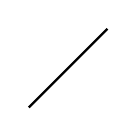
\begin{tikzpicture}[baseline=(P)] \draw[thick] (0,0) -- (1,1); \coordinate (P) at (0.5, 0.5); \end{tikzpicture} &
	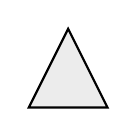
\begin{tikzpicture}[baseline=(P)] \filldraw[thick, fill=gray!15] (0,1) -- (-0.5, 0) -- (0.5, 0) --cycle; \coordinate (P) at (0, 0.5); \end{tikzpicture}
\end{tabular}\end{center}
三种构件粘成的空间; 要求点粘点, 边粘边, 如下情况是不容许的:
\begin{center}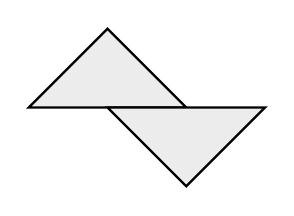
\begin{tikzpicture}[baseline=(O)]
	\filldraw[thick, fill=gray!15] (0,0) -- (1,1) -- (2,0)  --cycle;
	\filldraw[thick, fill=gray!15] (2, -1) -- (1,0) -- (3,0) --cycle;
	\coordinate (O) at (0,0);
\end{tikzpicture} \quad 不是单纯复形! \end{center}
相关定义详见 \cite[第六章]{You}. 高维情形的推广是自然的; 一般而言, 一个 $i$-维单纯形具有标准的实现
\[ \Delta^i := \left\{ (x_0, \ldots, x_i) \in \R^{i+1}_{\geq 0}: x_0 + \cdots + x_i = 1 \right\}, \]
其标准定向按法向量 $(1, \ldots, 1)$ 确定. 显见 $\Delta^i$ 的边界是一些 $j$-维单纯形的无交并 ($0 \leq j < i$). 如是分解中 $i-j$ 维的构件共有 $\binom{i+1}{j}$ 个, 相当于设其中 $j$ 个坐标为 $0$. 循此可以解释粘合的意义. 选定三角剖分相当于用组合办法确定一个空间的拓扑.

若单纯复形之间的连续映射 $\Phi: A \to B$ 映单纯形为单纯形 (容许降维), 并保持边界的粘合条件, 则我们说 $\Phi$ 是\emph{单纯映射}, 详见 \cite[第七章, \S 1]{You}.

\begin{lemma}\label{prop:Hurwitz-triangulation}
	设 $f: X \to Y$ 为紧 Riemann 曲面之间的非常值态射. 存在 $X, Y$ 的三角剖分, 使得
	\begin{compactitem}
		\item 剖分的每个单纯形都落在某个标准坐标卡中 (见命题 \ref{prop:morphism-ramified-covering} 证明), 而 $f$ 是单纯映射;
		\item $f(\mathrm{Ram}(f))$ 的每个元素都是 $Y$ 的顶点;
		\item $X$ 的剖分由 $Y$ 的点, 线, 面的原像给出, 每个线或面的原像都是 $\deg f$ 个线或面.
	\end{compactitem}
\end{lemma}
\begin{proof}
	取 $Y$ 的三角剖分, 充分加细使得离散集 $f(\mathrm{Ram}(f))$ 的元素皆为顶点, 而且每个单纯形都包含于某个标准坐标卡. 局部上化约到标准分歧复叠来观照 $f$, 概貌如下 (取 $e(x)=2$ 为例):
	\[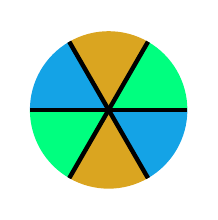
\begin{tikzpicture}[baseline=(X)]
		\coordinate (X) at (0,0);
		\fill[fill=SpringGreen] (0,0) -- (0:1) arc(0:60:1) --cycle;
		\fill[fill=SpringGreen] (0,0) -- (180:1) arc(180:240:1) --cycle;
		\fill[fill=Goldenrod] (0,0) -- (60:1) arc(60:120:1) --cycle;
		\fill[fill=Goldenrod] (0,0) -- (240:1) arc(240:300:1) --cycle;
		\fill[fill=Cerulean] (0,0) -- (120:1) arc (120:180:1) --cycle;
		\fill[fill=Cerulean] (0,0) -- (300:1) arc (300:360:1) --cycle;
		\foreach \x in {0, 60, ..., 300}
		\draw[ultra thick] (0,0) -- (\x:1);
	\end{tikzpicture} \quad \stackrel{w^2}{\longrightarrow} \quad
	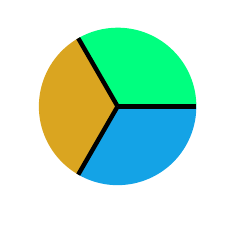
\begin{tikzpicture}[baseline=(Y)]
		\coordinate (Y) at (0,0);
		\fill[fill=SpringGreen] (0,0) -- (0:1) arc(0:120:1) --cycle;
		\fill[fill=Goldenrod] (0,0) -- (120:1) arc(120:240:1) --cycle;
		\fill[fill=Cerulean] (0,0) -- (240:1) arc (240:360:1) --cycle;
		\foreach \x in {0, 120, 240}
		\draw[ultra thick] (0,0) -- (\x:1);
	\end{tikzpicture}\]
	由此易见 $Y$ 的点, 线, 面的原像给出 $X$ 的三角剖分, 而 $f$ 对之成为单纯映射. 线和面的原像个数在标准分歧复叠情形是清楚的, 运用命题 \ref{prop:sum-ram-degree} 加总可得一般情形.
\end{proof}

接着回顾\emph{亏格}的概念. 精确到同胚, 可定向连通紧曲面 $S$ 由它们的亏格 $g = g(S)$ 完全分类; 直观上 $g$ 是曲面的洞数. 详见 \cite[第三章 \S 3.3]{You}. 如果取定了三角剖分, 则 $2 - 2g(S) = V(S) - E(S) + F(S)$, 其中 $V, E, F$ 分别是三角剖分中的点, 线, 面个数; 这个拓扑不变量称为 $S$ 的 \emph{Euler 示性数}, 记作 $\chi(S) := 2 - 2g(S)$. \index{kuige@亏格 (genus)} \index{Euler 示性数 (Euler characteristic)}

\[ S \quad \simeq \quad \underbrace{ 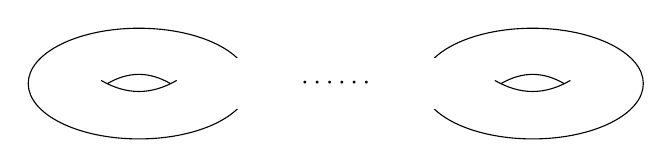
\begin{tikzpicture}[baseline=(T)]
	\coordinate (T) at (0,0);
	\begin{scope}[shift=(T), scale=0.4]
	\draw (-1,0) to [bend left] (1,0);
	\draw (-1.2,.1) to [bend right] (1.2,.1);
	\draw (0, 0) ellipse (100pt and 50pt);
	\fill[color=white] (2.8, -0.8) rectangle (4, 0.8);	% Erase
	\end{scope}
	\coordinate (S) at (5,0);
	\begin{scope}[shift=(S), scale=0.4]
	\draw (-1,0) to [bend left] (1,0);
	\draw (-1.2,.1) to [bend right] (1.2,.1);
	\draw (0,0) ellipse (100pt and 50pt);
	\fill[color=white] (-4, -0.8) rectangle (-2.8, 0.8);	% Erase
	\end{scope}
	\node at (2.5, 0) {$\cdots\cdots$};
	\end{tikzpicture} }_{g(S) \;\text{份}} \]

\begin{theorem}[Riemann--Hurwitz 公式]\label{prop:Riemann-Hurwitz} \index{Riemann--Hurwitz 公式}
	设 $f: X \to Y$ 为紧 Riemann 曲面之间的非常值态射, 则
	\[ 2g(X) - 2 = (2g(Y) - 2) \deg f + \sum_{x \in \mathrm{Ram}(f)} (e(x) - 1). \]
\end{theorem}
\begin{proof}
	对于任意三角剖分, 命题 \ref{prop:sum-ram-degree} 指出 $V(Y) \deg f = \sum_y \sum_{x \in f^{-1}(y)} e(x)$, 其中 $y$ 取遍 $Y$ 的顶点. 如运用引理 \ref{prop:Hurwitz-triangulation} 中的剖分, 这可改写作
	\begin{align*}
		V(X) & = \sum_{x: \text{顶点}} 1 = \sum_{y: \text{顶点}} \;\sum_{x \in f^{-1}(y)} 1 \\
		& = V(Y) \deg f - \sum_{x: \text{顶点}} (e(x) - 1),
	\end{align*}
	最后一项可以限制到 $x \in \text{Ram}(f)$ 上求和. 另一方面, 在引理 \ref{prop:Hurwitz-triangulation} 中已经说明
	\[ E(X) = E(Y) \deg f, \quad F(X) = F(Y) \deg f. \]
	用以上诸式计算 $\chi(X)$ 和 $\chi(Y)$ 即可.
\end{proof}

\section{全纯向量丛及其截面}\label{sec:vector-bundle}
在任意 Riemann 曲面乃至于复流形 $X$ 上都有\emph{全纯向量丛}的概念. 本书常略去全纯二字.

\begin{definition}
	在 $X$ 上,一个秩 $r \geq 1$ 的(全纯)向量丛是满足下述条件的连续映射 $\pi: E \to X$.
	\begin{itemize}
		\item $\pi$ 是局部平凡的: $X$ 有一族开覆盖 $\mathcal{U}$, 使得在每个开集 $U \in \mathcal{U}$ 上, 存在交换图表
		\[\begin{tikzcd}[row sep=small, column sep=small]
			E|_U := \pi^{-1}(U) \arrow[rr, "\varphi_U", "\sim"'] \arrow[rd, "\pi"'] & & U \times \CC^r \arrow[ld, "\text{pr}_1"] \\
			& U &
		\end{tikzcd}\]
		照例以 $\text{pr}_1$ 表示向第一个坐标投影, 而 $\varphi_U$ 是同胚. 称这样一族资料 $(U, \varphi_U)$ 为 $E$ 在开集 $U$ 上的\emph{平凡化}.
		\item 进一步, 对任意 $U, V \in \mathcal{U}$ 和 $\varphi_U, \varphi_V$ 如上, 定义转移映射 $\varphi_{VU}: \varphi_V \circ \varphi_U^{-1}: (U \cap V) \times \CC^r \to (U \cap V) \times \CC^r$; 我们要求
		\[ \varphi_{VU}(x,t) = (x,a_{VU}(x)t), \quad (x,t) \in (U \cap V) \times \CC^r, \]
		其中 $a_{UV}: U \cap V \to \GL(r,\CC)$ 是全纯函数 (即: 每个矩阵元都全纯). 这时也称 $(U, \varphi_U)$ 和 $(V, \varphi_V)$ 是相容的平凡化.
	\end{itemize}
	对任意开子集 $V \subset X$, 定义 $E$ 在 $V$ 上的(全纯)\emph{截面}为满足以下条件的映射 $V \xrightarrow{s} E$:
	\begin{compactitem}
		\item $\pi \circ s = \identity_V$;
		\item $s$ 全纯, 或者说一旦取定局部平凡化 $E|_U \xrightarrow[\sim]{\varphi_U} U \times \CC^r$, 则 $s|_U$ 表作 $(x, s_U(x))$, 其中 $s_U: U \to \CC^r$ 的每个坐标都是全纯函数.
	\end{compactitem}

	易验证条件无关局部平凡化的选取. 于是有 $\CC$-向量空间
	\index[sym1]{Gamma(V,E)@$\Gamma(V, E)$}
	\[ \Gamma(V, E) := \left\{ s: V \to E, \; \text{截面} \right\}, \]
	在局部平凡化 $\varphi_U$ 之下, 其向量空间结构由 $(a_1 s_1 + a_2 s_2)_U = a_1 s_{1,U} + a_2 s_{2,U}$ 反映 ($a_1, a_2 \in \CC$). 映射 $V \mapsto \Gamma(V, E)$ 给出对应到 $E$ 的\emph{截面层}.
\end{definition}

秩 $r$ 向量丛的截面层自然是 $\mathscr{O}_X$-模. 取局部平凡化可见截面层是秩 $r$ 局部自由 $\mathscr{O}_X$-模, 这在几何中是所谓凝聚层的一个例子.

称 $E$ 是丛的全空间, $X$ 是底空间. 一如流形情形, 我们习惯添入所有与 $\{(U, \varphi_U) : U \in \mathcal{U} \}$ 相容的局部平凡化, 以确保 $\{ (U, \varphi_U) : U \in \mathcal{U} \}$ 极大. 显见转移函数满足上链条件
\begin{gather*}
	\varphi_{UU} = \identity, \quad \text{或等价的} \quad a_{UU} = \identity; \\
	\varphi_{WV} \varphi_{VU} = \varphi_{WU}, \quad \text{或等价的}\quad a_{WV} a_{VU} = a_{WU}.
\end{gather*}
反过来说, 给定一族 $X$ 的开覆盖 $\mathcal{U}$ 及 $\{a_{VU}: U,V \in \mathcal{U} \}$ 满足如上条件, 由之可以粘合出向量丛 $\pi: E \to X$.

对每个 $x \in X$, 取 $U \ni x$ 上的局部平凡化, 从而 $\varphi_U: E_x := \pi^{-1}(x) \rightiso \{x\} \times \CC^r$ 使得纤维 $E_x$ 成为 $r$ 维复向量空间. 既然转移映射保持 $\CC^r \simeq \{x\} \times \CC^r$ 上的一切向量运算, $E_x$ 的向量空间结构无关 $(U,\varphi_U)$ 的选取. 所以 $E$ 可视作一族竖在 $X$ 上的 $r$ 维向量空间. ``丛''字明矣.

向量丛之间的态射 $\varphi: L_1 \to L_2$ 定义为使图表
$\begin{tikzcd}[row sep=small, column sep=tiny]
	L_1 \arrow[rr, "\varphi"] \arrow[rd] & & L_2 \arrow[ld] \\
	& X &
\end{tikzcd}$
交换, 并且局部形如 $(\identity, T_U): U \times \CC^r \to U \times \CC^s$ 的映射, 其中 $T_U: U \to \Hom_{\CC}(\CC^r, \CC^s) \simeq \CC^{rs}$ 的每个坐标都全纯; ``局部''自是相对于先前的平凡化 $\{\varphi_U\}_{U \in \mathcal{U}}$ 而言. 如此使得 $X$ 上的全体秩 $r$ 向量丛构成一范畴 $\mathsf{Vect}_r(X)$, 谈论向量丛的同构遂有意义.

形如 $X \times \CC^r \xrightarrow{\mathrm{pr}_1} X$ 的向量丛称为秩 $r$ 的\emph{平凡从}. 就底空间 $X$ 来看, 向量丛局部上都同构于平凡丛, 相应的同构由平凡化 $\varphi_U$ 给出.

线性代数的基本操作都可以搬到向量丛上. 以下 $E, F$ 表 $X$ 上的向量丛, $x \in X$ 是任意点.
\begin{center}\begin{tabular}{|r|c|c|c|c|} \hline
	& 对偶丛 & 直和丛 & 张量积丛 & 内 $\Hom$ 丛 \\ \hline
	符号 & $E^\vee$ & $E \oplus F$ & $E \otimes F$ & $\iHom(E, F) \simeq E^\vee \otimes F$ \\ \hline
	$x$ 上的纤维 & $(E_x)^\vee$ & $E_x \oplus F_x$ & $E_x \otimes F_x$ & $\Hom(E_x, F_x)$ \\ \hline
\end{tabular}\end{center}

举 $E^\vee$ 为例, 显然的办法是逐纤维地定义 $(E^\vee)_x := E_x^\vee$, 然后用 $E$ 的局部平凡化赋予 $E^\vee$ 向量丛结构. 其余构造类似, 无劳细说.

\begin{definition}
	给定 Riemann 曲面 (乃至于复流形, 不必假设连通) 的态射 $f: Y \to X$ 和秩 $r$ 向量丛 $\pi: E \to X$, 其\emph{拉回}定义为
	\[ f^* E := Y \times_X E = \left\{ (y, e) \in Y \times E: f(y) = \pi(e) \right\} \xrightarrow{\eta: \text{投影}} Y. \]

	考虑 $X$ 的一族开覆盖 $\mathcal{U}$ 和局部平凡化 $\varphi_U: E|_U \rightiso U \times \CC^r$, 其中 $U \in \mathcal{U}$. 由之自然地诱导出
	\[\begin{tikzcd}[row sep=small]
		\psi_U: \eta^{-1}(f^{-1}U) \arrow[r, "\sim"] & f^{-1}U \times \CC^r \\
		(y,e) \arrow[mapsto, r] & \left(y, \text{pr}_2 \varphi_U(e)\right) \\
		\left( y, \varphi_U^{-1}(f(y), t) \right) & (y, t) \arrow[mapsto, l]
	\end{tikzcd}\]
	此外 $Y = \bigcup_{U \in \mathcal{U}} f^{-1}U$. 由此可以验证 $f^*E \to Y$ 构成秩 $r$ 向量丛, 以 $(\psi_U)_{U \in \mathcal{U}}$ 为一族局部平凡化.
\end{definition}

例行的验证说明拉回和向量丛的种种操作相交换, 例如 $f^*(E_1 \oplus E_2) \simeq f^* E_1 \oplus f^* E_2$, $f^*(E_1 \otimes E_2) \simeq f^* E_1 \otimes f^* E_2$ 等等; 平凡丛拉回为平凡丛. 这些同构都具有函子性. 若 $f: U \hookrightarrow X$ 是开子集的包含映射, 则 $f^* E$ 无非是 $E$ 在 $U$ 上的限制.

\begin{definition}\index{xiancong@线丛 (line bundle)}
	秩 $r=1$ 的向量丛称为\emph{线丛}.
\end{definition}

平凡线丛的截面无非是全纯函数.

\begin{example}[重言式线丛]\label{eg:tautological-bundle} \index{xiancong!重言式 (tautological)}
	考虑例 \ref{eg:P1-cplx} 介绍的射影直线 $\PP^1 := \PP^1(\CC)$. 定义
	\[ \pi: \left\{ (x,v) \in \PP^1 \times \CC^2 : v \in x \right\} \to \PP^1, \quad \pi(x, v) = x. \]
	这是秩 $1$ 向量丛. 诚然, 考虑例 \ref{eg:P1-cplx} 的开覆盖 $\PP^1 = U_0 \cup U_1$, 那么可取
	\begin{center}\begin{tabular}{c|c}
			坐标卡 $U_0 := \{ (1:s) : s \in \CC \} \rightiso \CC$ & 坐标卡 $U_1 := \{(s:1) : s \in \CC \}$ \\ \hline
			$\begin{tikzcd}[row sep=small]
			\pi^{-1}(U_0) \arrow[r, "\sim"', "\varphi_0"] & U_0 \times \CC \\
			\left((1:s), (t,ts)\right) \arrow[r, mapsto] \arrow[phantom, u, "\in" sloped] & ((1:s), t); \arrow[phantom, u, "\in" sloped]
			\end{tikzcd}$ &
			$\begin{tikzcd}[row sep=small]
			\pi^{-1}(U_1) \arrow[r, "\sim"', "\varphi_1"] & U_1 \times \CC \\
			\left((s:1), (ts,t)\right) \arrow[r, mapsto] \arrow[phantom, u, "\in" sloped] & ((s:1), t). \arrow[phantom, u, "\in" sloped]
			\end{tikzcd}$
	\end{tabular}\end{center}
	
	现在来验证相容性: 记 $U_{01} := U_0 \cap U_1$, 以下交换图表说明 $a_{U_1 U_0}((a:b)) = \frac{b}{a}$.
	\[\begin{tikzcd}[column sep=0]
	& \pi^{-1}(U_{01}) \arrow[ld, "\varphi_0"'] \arrow[rd, "\varphi_1"] & \\
	(U_{01}) \times \CC \arrow[rr] \arrow[d, "\simeq"', "z_0"] & & (U_{01}) \times \CC \arrow[d, "\simeq", "z_1"'] \\
	\CC^\times \times \CC \arrow[rr, "\sim"] & & \CC^\times \times \CC \\
	(z, t) \arrow[mapsto, rr] \arrow[phantom, u, "\in" sloped] & & (z^{-1}, zt) \arrow[phantom, u, "\in" sloped]
	\end{tikzcd} \; \begin{tikzcd}[column sep=0]
	& \left( (a:b), (ta,tb) \right) \arrow[mapsto, ld] \arrow[mapsto, rd] & \\
	((a:b), ta) \arrow[mapsto, rr] \arrow[mapsto, d] & & ((a:b), tb) \arrow[mapsto, d] \\
	(\frac{b}{a}, ta) \arrow[mapsto, rr] & & (\frac{a}{b}, tb) \\
	\end{tikzcd}\]
	
	记此线丛为 $\mathscr{O}(-1)$. 任一点 $x \in \mathbb{P}^1$ 上的纤维无非 $x$ 这条线本身. 对于高维度的射影空间 $\mathbb{P}^n$ 乃至于更广的 Grassmann 簇也有类似的``重言式''构造.
\end{example}

\begin{exercise}
	说明 $\CC^2 \smallsetminus \{0\}$ 可以自然地嵌入丛 $\mathscr{O}(-1)$ 的全空间作为开子集.
\end{exercise}

留意到 $\GL(1,\CC) = \CC^\times$. 线丛的张量运算格外简单: 线丛的对偶与张量积仍是线丛; 对任意线丛 $\pi: L \to X$, 易见 $L^\vee \otimes L \simeq \iHom(L,L)$ 平凡, 而且对任意整数 $r$ 可以定义张量幂 $L^{\otimes r}$ 使之满足典范同构
\[ L^{\otimes r} \otimes L^{\otimes s} \simeq L^{\otimes (r+s)}, \quad L^{\otimes 0} \simeq \text{平凡线丛}, \quad L^{\otimes -1} \simeq L^\vee. \]
一如既往, 这些性质都化到一维向量空间情形来检验. 以例 \ref{eg:tautological-bundle} 的 $\mathbb{P}^1$ 上线丛 $\mathscr{O}(-1)$ 为例, 一般记
\[ \mathscr{O}(r) := \mathscr{O}(-1)^{\otimes (-r)} = \mathscr{O(1)}^{\otimes r}, \quad r \in \Z. \]
可以证明 $\mathbb{P}^1$ 上的线丛都同构于某个 $\mathscr{O}(r)$, 其中 $r \in \Z$ 是唯一的; 我们不需要这个结果.

若在线丛截面的定义中容许 $s_U$ 为亚纯函数, 便得到 $L$ 的\emph{亚纯截面}. 例如平凡线丛的亚纯截面无非是亚纯函数. 根据线丛定义中的相容性条件, 变动 $L$ 的局部平凡化相当于代 $s_U(x)$ 为 $s_U(x) \alpha_U(x)$, 其中 $\alpha_U: U \to \CC^\times$ 全纯, 这不改变任意点 $x \in U$ 处的 $\ord_x(s_U)$. 以下因之是良定的.

\begin{definition}\label{def:vanishing-order-section} \index{xiaomeicishu} \index[sym1]{ord}
	对于 $x \in X$ 和线丛 $L$ 在 $x$ 附近的亚纯截面 $s$, 选取充分小的开邻域 $U \ni x$, 任选 $L$ 的局部平凡化以定义 $s$ 在 $x$ 处的消没次数 $\ord_x(s) := \ord_x(s_U)$. 特别地, 我们可以谈论 $s$ 的极点和零点, 及其重数.
\end{definition}

运用线丛的局部平凡化, 容易化约到亚纯函数情形来验证下述性质
\begin{equation}\label{eqn:ultrametric-valuation}
	\ord_x(s_1 + s_2) \geq \min\left\{ \ord_x(s_1), \ord_x(s_2) \right\}, \quad s_1, s_2: L\; \text{在 $x$ 附近的亚纯截面}.
\end{equation}

我们最关心的是一些源自 $X$ 自身的几何结构, 并且携带丰富信息的线丛. 以下是一个至关紧要的情形.
\begin{definition}[典范丛]\label{def:canonical-bundle}
	\index{dianfancong@典范丛 (canonical bundle)} \index{quanchunweifen@全纯微分 (holomorphic differential)} \index{yachunweifen@亚纯微分 (meromorphic differential)} \index[sym1]{OmegaX@$\Omega_X$}
	全纯余切从 $\Omega_X := T^*_\text{hol}(X)$ 是秩 $1$ 的, 称为 $X$ 的\emph{典范丛}, 其全纯截面在局部坐标卡下总能表为 $f \dd z$ 之形, 其中 $f: U \to \CC$ 全纯, $U \subset X$ 为带有局部坐标 $z$ 的开集. 探讨亚纯截面相当于容许 $f$ 为亚纯函数.
	
	习惯称 $\Omega_X$ 的亚纯截面为 $X$ 上的\emph{亚纯微分}, 称其全纯截面为\emph{全纯微分}.
\end{definition}

进一步, 对任意 $r \in \Z$ 都有张量幂 $\Omega_X^r := \Omega_X^{\otimes r}$, 而 $\Omega_X^{-1} = \Omega_X^\vee$ 无非是 $X$ 的全纯切丛 $T_\text{hol} X$.

\begin{example}\label{eg:canonical-bundle-P1}
	取 $X = \mathbb{P}^1$. 沿用例 \ref{eg:P1-cplx} 的坐标卡 $(U_i, z_i)_{i=0,1}$; 在 $U_0 \cap U_1$ 上 $z_0 = z_1^{-1}$. 取微分得到 $\Omega_{\mathbb{P}^1}|_{U_0 \cap U_1}$ 中的等式
	\[ \dd z_0 = -z_1^{-2} \dd z_1 = -z_0^2 \dd z_1. \]

	现在分别在 $U_0, U_1$ 上用 $\dd z_0$ 和 $-\dd z_1$ 将 $\Omega_X$ 平凡化, 可见转移函数为 $a_{U_1 U_0}(a:b) = z_0(a:b)^2 = \left(\frac{b}{a}\right)^2$. 与例 \ref{eg:tautological-bundle} 比较, 立见
	\[ \Omega_{\mathbb{P}^1} \simeq \mathscr{O}(-1)^{\otimes 2} = \mathscr{O}(-2). \]
\end{example}

\begin{example}\label{eg:canonical-bundle-tori}
	任意复环面 $A \simeq \CC/\Lambda$ 的典范丛都具有自然的平凡化. 这点是群结构的直接应用: 在 $0 \in A$ 的全纯余切空间上任选一个非零元 $\omega$. 对任意 $x \in A$, 平移映射 $t \mapsto x+t$ 给出自同构 $L_x: A \rightiso A$; 连带地, $\omega(x) := (L_{-x})^* \omega$ 定义了 $\Omega_A$ 的一个处处非零的全纯截面 $x \mapsto \omega(x)$. 如是遂有同构
	\begin{align*}
		\Omega_A = T^*_{\text{hol}} A & \stackrel{\sim}{\longleftarrow} A \times \CC \\
		\left[ t\omega(x) \in T^*_{\text{hol}, x} A \right] & \longmapsfrom (x, t).
	\end{align*}
\end{example}

考虑 Riemann 曲面的态射 $f: Y \to X$. 相应地有向量丛的自然态射
\begin{align*}
	f^* \Omega_X = Y \times_X \Omega_X & \longrightarrow \Omega_Y \\
	(y, \omega) & \longmapsto f^* \omega
\end{align*}
这里 $\omega \in T^*_{f(y), \text{hol}}$, 它自然地拉回到 $f^* \omega \in T^*_{y, \text{hol}}$, 见 \S\ref{sec:Riemann-basics}. 所以 $f^* \Omega_X \to \Omega_Y$ 确实良定. 进一步, 可以对任意 $k \in \Z$ 考虑相应的 $f^* \Omega_X^{\otimes k} \to \Omega_Y^{\otimes k}$.

\section{亚纯微分的应用}
留数定理对于一般的 Riemann 曲面 $X$ 依然成立. 其中涉及围道积分和留数, 其正确表述都需要微分形式的语言. 首先, 对于 $X$ 上的亚纯微分 $\omega$ 和分段光滑曲线 $C: [0,1] \to X$, 只要 $\omega$ 在 $C$ 的像里无极点, 道路积分 $\int_C \omega = \int_0^1 C^* \omega$ 总是有定义的. 另一方面, $\omega$ 在任一点 $x$ 的留数 $\Res_x(\omega)$ 也有定义. 两种定义都只依赖于 $\omega$, 无关坐标; 关于 $\int_C \omega$ 的情形, 各位在学习流形上的微积分时应该有所心得, 至于 $\Res_x \omega$ 的良定性, 归根结柢出自以下观察.

首先, 对不恒为 $0$ 的亚纯函数 $f$ 可定义亚纯微分 $\dd\log f = \frac{\dd f}{f}$, 它在任意局部坐标 $z$ 下表成 $f^{-1} \frac{\dd f}{\dd z} \dd z$.

接着在 $x$ 附近取坐标 $z$ 使得 $z(x)=0$. 考虑亚纯微分形式 $\omega$ 在 $z=0$ 附近的 Laurent 展开 $\sum_{k > -\infty} a_k z^k \dd z$. 在这类展开式组成的向量空间中, 我们 $\bmod$ 掉
\begin{compactenum}[(a)]
	\item 定义在 $z = 0$ 附近的全纯微分形式,
	\item 形如 $\dd\eta$ 的微分形式, 其中 $\eta$ 是定义在 $z = 0$ 附近的亚纯函数.
\end{compactenum}
得到的商空间记为 $\mathcal{R}$, 无关坐标 $z$ 的选取; 记 $\omega$ 在 $\mathcal{R}$ 中的像为 $[\omega]$. 取商相当于舍去 Laurent 展开中 $k \neq -1$ 的项, 因之 $\dd\log z$ 的像是一维空间 $\mathcal{R}$ 的基, $[\omega]$ 对之的系数正是 $a_{-1} = \Res_x(\omega)$. 为了说明 $\Res_x(\omega)$ 独立于坐标, 只消说明 $\dd\log z$ 在 $\mathcal{R}$ 中的像独立于 $z$. 诚然, 对于任两个满足 $z(x) = 0 = w(x)$ 的局部坐标 $z, w$, 形式操作给出 $\dd\log z - \dd\log w = \dd\log \dfrac{z}{w}$, 而 $\dfrac{z}{w}$ 在 $x = 0$ 附近非零, 故 $\dd \log z \equiv \dd \log w \pmod{\text{全纯微分}}$.

\begin{lemma}\label{prop:res-ord}
	设 $f$ 是亚纯函数, 不处处为零, 则对任意 $x \in X$ 皆有 $\mathrm{ord}_x(f) = \Res_x\left( \dd\log f \right)$.
\end{lemma}
\begin{proof}
	取局部坐标 $z$ 使得 $z(x)=0$, 直接计算 $\dd \log f = f^{-1} \frac{\dd f}{\dd z}$ 的留数.
\end{proof}

\begin{theorem}\label{prop:contour-Res}
	设 $D$ 是 $X$ 中的紧区域, 边界 $\partial D$ 是分段光滑曲线, 带诱导定向, 而亚纯微分 $\omega$ 在 $\partial D$ 上无极点, 则
	\[ \frac{1}{2\pi i} \oint_{\partial D} \omega = \sum_{\substack{x \in D^\circ \\ \text{极点}}} \Res_x(\omega). \]
\end{theorem}
边界 $\partial D$ 的诱导定向来自 $D$ 本身由复结构确定的定向. 在局部坐标卡下, 这相当于说 $\partial D$ 逆时针绕行, 如下图.
\begin{center}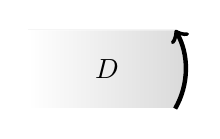
\begin{tikzpicture}
	\fill[draw=white, shading=axis, right color=gray!30, left color=white] (-1, -0.5) -- (-30:1) arc(-30:30:1) -- (-1, 0.5) --cycle;
	\draw[ultra thick, ->] (-30:1) arc(-30:30:1);
	\node at (0,0) {$D$};
\end{tikzpicture}\end{center}
定理中容许 $\partial D = \emptyset$ (例如 $D=X$), 空曲线上的围道积分定为 $0$.
\begin{proof}
	如果 $D$ 能用 $X$ 的一个局部坐标卡覆盖, 那这无非是经典的留数定理. 一般情形下, 取足够细的三角剖分 $D = D_1 \cup \cdots \cup D_m$ 以确保每个 $D_i$ 都能用坐标卡覆盖, 适加扰动以确保 $\bigcup_i \partial D_i$ 不包含 $\omega$ 的极点. 剖分新添的边积分相消, 由此立刻化约到前一情形.
	
	这些论证在边界为空时同样适用, 以复环面 $X = D = \CC\big/(\Z \oplus \Z i)$ 为例, 图像如下:
	\[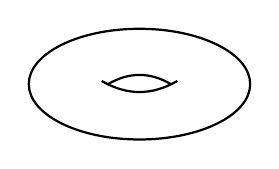
\begin{tikzpicture}[baseline=(T), every path/.style={thick}]
		\coordinate (T) at (0,0);
		\begin{scope}[shift=(T), scale=0.4]
		\draw (-1,0) to [bend left] (1,0);
		\draw (-1.2,.1) to [bend right] (1.2,.1);
		\draw (0, 0) ellipse (100pt and 50pt);
		\end{scope}
	\end{tikzpicture} \; \xleftarrow[\text{基本区域}]{\text{粘合}} \;
	\begin{tikzpicture}[baseline=(R)]
		\coordinate (R) at (1, 1);
		\fill[color=gray!20] (0,0) rectangle (2,2);
		\draw[color=blue, ultra thick] (0,0) -- (2,0);
		\draw[color=blue, ultra thick] (0,2) -- (2,2);
		\draw[color=red, ultra thick] (0,0) -- (0,2);
		\draw[color=red, ultra thick] (2,0) -- (2,2);
		\begin{scope}[shift=(R)]
			\draw[-Latex, thick] (20:0.4) arc (20:340:0.4);
		\end{scope}
	\end{tikzpicture} \quad \stackrel{\text{剖分}}{=} \quad
	\begin{tikzpicture}[baseline=(S3), every path/.style={draw, ultra thick, arrows = {-Latex[scale length=0.5] . Latex[scale length=0.5]}}]
		\coordinate (S1) at (0, 0);
		\coordinate (S2) at (0, 0.5);
		\coordinate (S3) at (0, .75);
		\begin{scope}[shift=(S1)]
			\fill[gray!20] (0,0) -- (2,0) -- (2,1) --cycle;
			\draw (0,0) -- (2,0); \draw (2,0) -- (2,1); \draw (2,1) -- (0,0);
		\end{scope}
		\begin{scope}[shift=(S2)]
			\fill[gray!20] (0,0) -- (2,1) -- (0,1) --cycle;
			\draw (0,0) -- (2,1); \draw (2,1) -- (0,1); \draw (0,1) -- (0,0);
		\end{scope}
	\end{tikzpicture}\]
	各边的积分两两相消. 
\end{proof}

\begin{theorem}\label{prop:sum-of-residues}
	设 $X$ 为紧 Riemann 曲面.
	\begin{enumerate}[(i)]
		\item 对任意亚纯微分 $\omega$ 皆有 $\sum_x \Res_x(\omega) = 0$, 其中 $x$ 取遍极点;
		\item 对任意不恒为零的亚纯函数 $f$,
		\[ \sum_{x \in X} \mathrm{ord}_x(f) = 0 \quad \text{(有限和)}, \]
		或者说 $f$ 的极点与零点的个数相同, 计入重数.
	\end{enumerate}
\end{theorem}
\begin{proof}
	定理 \ref{prop:contour-Res} 给出 (i), 代入亚纯微分 $\omega := \dd\log f$ 并应用引理 \ref{prop:res-ord} 就得到 (ii).
\end{proof}

设 $f$ 为 $X$ 上的非常值亚纯函数. 对任意 $y \in \CC \sqcup \{\infty\}$, 当 $y \neq \infty$ 时定义 $f$ 取 $y$ 值的次数为 $f-y$ 的零点个数, 若 $y=\infty$ 则定之为 $f$ 的极点个数; 当然, 两种情形下都计入重数, 见定义 \ref{def:vanishing-order}.

\begin{corollary}\label{prop:value-degree}
	非常值亚纯函数取 $y \in \CC \sqcup \{\infty\}$ 值的次数是一个无关 $y$ 的常数 $n(f) \in \Z_{\geq 1}$. 如果视 $f$ 为态射 $X \to \PP^1$, 则 $n(f)$ 无非是此态射的次数.
\end{corollary}
\begin{proof}
	当 $y \in \CC$, 在定理 \ref{prop:sum-of-residues} 中代入 $f-y$ 可知: (以下皆计重数)
	\begin{gather*}
		(\text{$f$ 取 $y$ 值的次数}) - (\text{$f$ 的极点个数}) = \\
		(\text{$f-y$ 的零点个数}) - (\text{$f-y$ 的极点个数}) = 0.
	\end{gather*}
	然而 $f$ 的极点数又等于 $f$ 取 $\infty$ 值的次数, 记为 $n(f) := \sum_{x \in f^{-1}(\infty)} -\text{ord}_x(f)$. 这就说明取 $f$ 取 $y \in \CC \sqcup \{\infty\}$ 值的次数是常数 $n(f)$.
	
	现将 $f$ 视同态射 $X \to \PP^1$. 兹断言 $\deg(f) = n(f)$. 以下用 $f$ 的零点个数 (计重数) 来计算 $n(f)$. 在每个 $x \in f^{-1}(0)$ 附近存在局部坐标 $w$ 使得 $f = w^{e(x)}$, 其中 $e(x) \geq 1$ 是 $x$ 处的零点重数. 根据注记 \ref{rem:ramification-index} 可知 $e(x)$ 正是 $f: X \to \PP^1$ 在 $x$ 处的分歧指数. 如是遂有
	\[ n(f) = \text{零点个数} = \sum_{x \in f^{-1}(0)} e(x) = \deg\left(X \xrightarrow{f} \PP^1 \right); \]
	最末等号基于命题 \ref{prop:sum-ram-degree}. 明所欲证.
\end{proof}

\begin{example}\label{eg:P1-meromorphic}
	且看如何用定理 \ref{prop:sum-of-residues} 来刻画射影直线 $\PP^1 \xrightarrow[\sim]{t} \CC \sqcup \{\infty\}$ 上的亚纯函数. 我们断言
	\[ \mathcal{M}(\PP^1) = \CC(t) \quad \text{(一元有理函数域)}. \]
	
	易见 $\CC(t) \subset \mathcal{M}(\PP^1)$. 若 $f,g \in \CC[t]$, $g \neq 0$, 基于极限的论证给出 $-\text{ord}_\infty\left( \dfrac{f}{g} \right) = \deg f - \deg g$, 这个次数差可以合理地记为 $\deg(f/g)$. 现在来证明任意 $h \in \mathcal{M}(\PP^1)^\times$ 皆为有理函数. 命
	\[ k(t) := \prod_{x \in \CC} (t - x)^{\text{ord}_x(h)} \; \in \CC(t) \quad \text{(有限积)}. \]
	
	由定理 \ref{prop:sum-of-residues} 导出
	\[ -\text{ord}_\infty(k) = \deg(k) = \sum_{x \in \CC} \text{ord}_x(h) = -\text{ord}_\infty(h), \]
	是以命题 \ref{prop:holomorphic-const} 蕴涵 $k/h$ 为常数. 综之, $h \in \CC(t)$.
\end{example}

\section{Riemann--Roch 定理的陈述}\label{sec:RR}
本节选定连通紧 Riemann 曲面 $X$, 其上的亚纯函数域仍记为 $\mathcal{M}(X)$.

\begin{definition}
	\index{chuzi@除子 (divisor)} \index[sym1]{Div-div@$\Div(X), \divisor(f)$}
	由 $X$ 的点生成的自由交换群记为 $\Div(X)$, 其元素称为 $X$ 上的\emph{除子}, 形式地表作有限和
	\[ D = \sum_{x \in X} n_x x, \quad n_x \in \Z, \quad \text{至多有限个 $n_x$ 非零.} \]
	相应的代数运算记为 $\sum_x n_x x \pm \sum_x m_x x = \sum_x (n_x \pm m_x)x$ 等等. 定义一个除子 $D = \sum_x n_x x$ 的\emph{次数}为
	\[ \deg D := \sum_{x \in X} n_x \; \in \Z. \]
	显然 $\deg: \Div(X) \to \Z$ 是群同态. 对于 $f \in \mathcal{M}(X)^\times$, 定
	\[ \divisor(f) := \sum_{x \in X} \ord_x(f) x \; \in \Div(X); \]
	形如 $\divisor(f)$ 的除子称为\emph{主除子}.
\end{definition}

全体主除子构成 $\Div(X)$ 的子群 $\mathcal{P}$. 事实上,
\[ \divisor(fg) = \divisor(f)+\divisor(g), \quad \divisor(f^{-1}) = -\divisor(f), \quad \divisor(c)=0, \; c \in \CC^\times .\]
\begin{definition}\label{def:Picard-group} \index{chuzileiqun@除子类群 (divisor class group)} \index{Picard 群} \index[sym1]{PicX@$\Pic(X)$}
	称商群 $\Pic(X) := \Div(X)/\mathcal{P}$ 为 $X$ 的\emph{除子类群}, 也称为 Picard 群.
\end{definition}

\begin{lemma}\label{prop:Pic-degree}
	对任意 $D \in \mathcal{P}$ 皆有 $\deg D = 0$. 因之 $\deg$ 诱导出群同态 $\Pic(X) \to \Z$.
\end{lemma}
\begin{proof}
	应用定理 \ref{prop:sum-of-residues}.
\end{proof}

\begin{example}\label{eg:Pic-P1}
	我们断言 $\deg$ 诱导同构 $\Pic(\PP^1) \rightiso \Z$. 仅须证明所有 $x \in \PP^1$ 皆满足 $x - \infty \in \mathcal{P}$ 即可, 因如此一来所有除子 $D$ 在 $\Pic(X)$ 中的类皆可化作 $n\infty$ 之形, 而 $\deg(n\infty) = n$. 诚然, 设 $x \neq \infty$, 考虑有理函数 $f = (t - x) \in \CC(t)$; 回忆例 \ref{eg:P1-meromorphic} 中的讨论可知 $\divisor(f) = t - \infty$, 证毕.
\end{example}

紧接着要考虑 $X$ 上的全纯线丛, 简称线丛, 以及它们的截面; 详见 \S\ref{sec:vector-bundle}.

\begin{theorem}\label{prop:meromorphic-section}
	在 $X$ 上, 任何线丛 $\pi:L \to X$ 都有非零的亚纯截面.
\end{theorem}
这点是由 $X$ 的紧性确保的. 其证明需要进一步的分析学工具, 且置不论.

\begin{definition-theorem}\label{def:div-L-s}
	设 $s$ 是线丛 $L$ 的亚纯截面, 不恒为 $0$. 定义相应的除子
	\[ \divisor(L, s) := \sum_{x \in X} \ord_x(s) x \; \in \Div(X). \]
	它在 $\Pic(X)$ 中的除子类不依赖 $s$ 的选取, 记为 $[L]$. 综之得到交换图表
	\[\begin{tikzcd}
		(L,s) \arrow[mapsto, r] \arrow[phantom, d, "\in" sloped] & \divisor(s) \arrow[phantom, d, "\in" sloped] \\
		\left\{ (L,s): L \to X\; \text{线丛},\; s \neq 0: \text{亚纯截面} \right\} \big/ \simeq \arrow[r] \arrow[d, "\text{忘记 $s$}"'] & \Div(X) \arrow[twoheadrightarrow, d, "\text{商}"] \\
		\left\{ L \to X: \; \text{线丛} \right\} \big/ \simeq \arrow[r] & \Pic(X) \\
		L \arrow[mapsto, r] \arrow[phantom, u, "\in" sloped] & {[L]} \arrow[phantom, u, "\in" sloped]
	\end{tikzcd}\]
	此处定义 $\varphi: (L,s) \rightiso (L',s')$ 为同构, 如果 $\varphi: L \rightiso L'$ 是线丛的同构且 $\varphi s = s'$.
\end{definition-theorem}
\begin{proof}
	首先, 在局部坐标下容易验证 $s$ 的极点与零点都是 $X$ 的离散子集, 从而 $\divisor(L,s)$ 确实定出 $\Div(X)$ 的元素. 今选定 $L$, 设亚纯截面 $s, s'$ 俱非零, 则在每个局部坐标邻域 $U$ 里总存在 $U$ 上不恒为 $0$ 的亚纯函数 $a_U$,
	\[ s'|_U = a_U s|_U, \quad a_U|_{U \cap V} = a_V|_{U \cap V}. \]
	从而 $(a_U)_U$ 粘合为 $a \in \mathcal{M}(X)$ 使得 $s' = as$. 按定义可知
	\[ \divisor(L,s') = \divisor(L,as) = \divisor(a) + \divisor(L,s) \in \mathcal{P} + \divisor(L,s), \]
	故 $\divisor(L,s)$ 的除子类 $[L]$ 仅依赖于 $L$. 这些构造显然在同构下不变.
\end{proof}

若 $L$ 是平凡线丛, 考虑常值截面 $s=1$ 立见 $[L]=0$.

如果 $s, s' \neq 0$ 分别是线丛 $L$, $L'$ 的亚纯截面, 那么可以构造 $L \otimes L'$ 的亚纯截面 $ss' = s \otimes s'$, 下述结果是水到渠成的.
\begin{proposition}\label{prop:class-L-additivity}
	我们有 $\divisor(L \otimes L', ss') = \divisor(L,s) + \divisor(L',s')$. 特别地, $[L \otimes L'] = [L] + [L']$, 且 $\left[ L^{\otimes r} \right] = r[L]$, 其中 $r \in \Z$.
\end{proposition}
\begin{proof}
	第一个等式可直接检验. 一并注意到 $L$ 及其对偶 $L^\vee$ 的张量积同构于平凡线丛, 于是 $[L] + [L^\vee] = 0$, 其余是明显的.
\end{proof}

\begin{example}\label{eg:P1-divisor-class}
	在 $\PP^1$ 上有 $[\mathscr{O}(r)] = rP$, 其中 $P \in \PP^1$ 是任意点, 不影响除子类 (见例 \ref{eg:Pic-P1}). 根据命题 \ref{prop:class-L-additivity}, 证 $r=1$ 的情形即足. 以下将用全纯截面来计算 $[\mathscr{O}(1)]$.

	既然 $\mathscr{O}(-1)$ 在任一点 $x$ 上的纤维是 $x$ 这条直线, 给定 $\mathscr{O}(1)$ 的全纯截面相当于为每个 $x \in \PP^1$ 指派 $x$ 上的一个线性泛函 $\lambda_x$, 并要求 $\lambda_x$ 随 $x$ ``全纯地''变化. 一个明显的取法是令 $\lambda$ 为 $\CC^2$ 上的线性泛函, 并且令 $\lambda_x := \lambda|_x$; 这对 $x$ 当然是全纯的, 它甚且是``代数的''.

	显然, 当 $\lambda \neq 0$ 时 $x \mapsto \lambda|_x$ 唯一的零点是 $x = \Ker(\lambda) \in \PP^1$. 为了计算重数, 不妨就取 $\lambda(a,b) = a$, 于是 $\Ker(\lambda)=(0:1)$. 在坐标开集 $U_1 = \{ (z:1) : z \in \CC \}$ 上, $\mathscr{O}(1)$ 有平凡化
	\[\begin{tikzcd}[row sep=small]
		U_1 \times \CC \arrow[r, "\sim"] & \left\{ ((z:1), \mu_z) : \mu_z \in \Hom_{\CC}\left( \CC  \cdot (z,1), \; \CC\right) \right\} \\
		((z:1), t) \arrow[r, mapsto] \arrow[phantom, u, "\in" sloped] & \left((z:1), (uz,u) \mapsto  ut \right). \arrow[phantom, u, "\in" sloped]
	\end{tikzcd}\]
	故 $\lambda|_{(z:1)}: (uz,u) \mapsto uz$ 对应到左侧平凡线丛的截面 $z \mapsto ((z:1), z)$, 它在 $z=0$ 处有一阶零点, 对应到 $(0:1) \in \PP^1$. 综之, $\divisor(\mathscr{O}(1), x \mapsto \lambda|_x) = (0:1)$, 证毕.
\end{example}

我们研究亚纯截面的进路是约束其极点, 借以获取一个``有限''的对象. 引入符号
\[ D = \sum_x n_x x, \; D' = \sum_x n'_x x, \quad D \geq D' \iff \left[ \forall x \in X, \; n_x \geq n'_x \right]. \]
对任意除子 $D$, 置 \index[sym1]{Gamma(X, L(D))@$\Gamma(X, L(D))$}
\[ \Gamma(X, L(D)) := \left\{ s: L\; \text{的亚纯截面}, \quad \divisor(L,s) + D \geq 0 \right\}. \]
按约定, $s = 0$ 给出 $\sum_x \infty x$, 属于上述集合. 易见 $\Gamma(X, L(D))$ 构成复向量空间, 见 \eqref{eqn:ultrametric-valuation}. 一般而言, $D \geq D'$ 蕴涵 $\Gamma(X, L(D')) \subset \Gamma(X, L(D))$, 而且易见 $\Gamma(X, L(0)) = \Gamma(X, L)$.

当 $L$ 平凡时, $\Gamma(X, L(D))$ 化为
\begin{equation}\label{eqn:Gamma-D}
	\Gamma(X, D) := \left\{ a \in \mathcal{M}(X) : \divisor(a) + D \geq 0 \right\}.
\end{equation}
按先前关于 $\divisor(0)$ 的约定, $\Gamma(X, D)$ 是 $\mathcal{M}(X)$ 的复向量子空间. 精确到同构, $\Gamma(X,D)$ 仅依赖于 $D$ 的除子类, 这是基于以下事实
\begin{equation}\label{eqn:C-section-invariance}\begin{tikzcd}[row sep=small]
	\Gamma(X, D) \arrow[r, "\sim"] & \Gamma(X, D + \divisor(f)), & f \in \mathcal{M}(X)^\times \\
	a \arrow[mapsto, r] \arrow[phantom, u, "\in" sloped] & af^{-1}. \arrow[phantom, u, "\in" sloped] &
\end{tikzcd}\end{equation}

\begin{lemma}\label{prop:low-degree-vanishing}
	当 $D=0$ 时 $\Gamma(X,D) = \CC$. 当 $\deg D < 0$ 时 $\Gamma(X,D) = \{0\}$.
\end{lemma}
\begin{proof}
	若 $D=0$ 则 $\Gamma(X,D)$ 是 $X$ 上的全纯函数空间. 由命题 \ref{prop:holomorphic-const} 知全纯函数必取常值.	现在证明后半部. 若 $a \in \mathcal{M}(X)^\times$, $\divisor(a) + D \geq 0$, 则 $\deg(\divisor(a) + D) = \deg D \geq 0$.
\end{proof}

空间 $\Gamma(X, L(D))$ 与 $\Gamma(X, D)$ 有紧密的联系.
\begin{proposition}\label{prop:C-section-L}
	设 $s$ 是线丛 $ L \to X$ 的亚纯截面, 不恒为零, 则对任意 $D \in \Div(X)$ 皆有同构
	\[\begin{tikzcd}[row sep=small, column sep=small]
		\Gamma(X, L(D)) \arrow[r, "\sim"] & \Gamma(X, \divisor(L,s) + D) & \\
		t = as \arrow[mapsto, r] \arrow[phantom, u, "\in" sloped] & a \arrow[phantom, u, "\in" sloped] & a \in \mathcal{M}(X).
	\end{tikzcd}\]
\end{proposition}

根据 \eqref{eqn:C-section-invariance}, 同构意义下 $\Gamma(X, \divisor(L,s) + D)$ 由 $\divisor(L,s)$ 的除子类亦即 $[L]$ 所确定, $s$ 的选取无关宏旨.
\begin{proof}
	任何 $L$ 的亚纯截面 $t$ 总能唯一地表作 $t=as$, 其中 $a \in \mathcal{M}(X)$; 见定义--定理 \ref{def:div-L-s} 的论证. 于是 $\divisor(L,t)+D \geq 0$ 等价于 $\divisor(a) + \divisor(L,s) + D \geq 0$. 证毕.
\end{proof}

\begin{definition} \index{dianfancong}
	\index[sym1]{l(D)@$\ell(D)$} \index[sym1]{KX@$K_X$}
	今对任意除子 $D \in \Div(X)$ 定义
	\[ \ell(D) := \dim_{\CC} \Gamma(X, D); \]
	根据 \eqref{eqn:C-section-invariance} 它只依赖于 $D$ 在 $\Pic(X)$ 中的类. 此外, 以 $X$ 的典范丛 (定义 \ref{def:canonical-bundle}) 定义\emph{典范除子类}
	\[ K_X := [\Omega_X] \; \in \Pic(X). \]
	于命题 \ref{prop:C-section-L} 代入 $L = \Omega_X$ 和 $D=0$ 可知 $\dim \Gamma(X, \Omega_X) = \ell(K_X)$.
\end{definition}
举例明之, $K_{\PP^1} = -2x \mod \mathcal{P}$, 其中 $x \in \PP^1$ 任取 (例 \ref{eg:P1-divisor-class} 配合例 \ref{eg:canonical-bundle-P1}). 另一方面, 对任意复环面 $T$ 都有 $K_T = 0$ (例 \ref{eg:canonical-bundle-tori}).

因为 $X$ 是紧定向曲面, 对之可定义亏格 $g = g(X)$ 和 Euler 示性数 $\chi(X) = 2 - 2g(X)$. 详见 \S\ref{sec:Riemann-Hurwitz}.

\begin{theorem}[Riemann--Roch]\label{prop:RR} \index{Riemann--Roch 定理}
	对任意除子 $D$, 维数 $\ell(D)$ 总是有限. 进一步
	\[ \ell(D) - \ell(K_X - D) = \deg D - g + 1. \]
\end{theorem}

这些论断的证明一般须动用称为 Hodge 理论的分析学工具, 宜待专著讨论, 感兴趣的读者不妨参阅 \cite[第三章]{Mei13}. 对于一般的紧复流形上的全纯向量丛, 相应的推广称为 Hirzebruch--Riemann--Roch 定理. 现在知道这是 Atiyah--Singer 指标定理的一个应用. 指标定理可谓进路迭出, 异彩纷呈, 读者从 \cite[Theorem 4.10]{BGV04} 切入兴许是个可行的方案.

\begin{remark}\label{rem:RR}
	下面是定理 \ref{prop:RR} 的几点立即推论.
	\begin{enumerate}
		\item 取 $D=0$, 由 $\ell(D) = \dim_{\CC} \CC = 1$ 和 $\deg D = 0$ 立得 $\ell(K_X) = g$.
		\item 复取 $D=K_X$, 配合上一步可知 $g-1 = \deg K_X - g + 1$, 亦即 $\deg K_X = 2g - 2 = -\chi(X)$.
		\item 若 $\deg D > 2g-2$, 则 $\deg(K_X-D) = \deg K_X - \deg D < 0$ 和引理 \ref{prop:low-degree-vanishing} 蕴涵 $\ell(K_X-D) = 0$, 从而
		\[ \ell(D) = \deg D - g + 1 > g-1; \]
		特别地, 假设 $\deg D > 2g-2$, 则当 $g \geq 1$ 时 $\ell(D) > 0$. 当 $g=0$ 而 $\deg D \geq 0$ 时也有 $\ell(D) > 0$.
	\end{enumerate}
\end{remark}

\begin{corollary}
	在 $X$ 上存在非零全纯微分当且仅当 $X$ 的亏格 $g \geq 1$.
\end{corollary}
\begin{proof}
	以上讨论表明 $\dim_{\CC} \Gamma(X, \Omega_X) = \ell(K_X) = g$.
\end{proof}

经常同 Riemann--Roch 定理合并运用的一个基本结果是 \emph{Serre 对偶定理}, 涉及向量丛或凝聚层的上同调, 记录如下.
\begin{theorem}[J.-P.\ Serre]\label{prop:Serre-duality} \index{Serre 对偶定理 (Serre duality)}
	存在 $\CC$-向量空间的自然同构
	\[ \Hm^i\left(X, E\right) \rightiso \Hm^{1-i}\left(X, E^\vee \otimes \Omega_X \right)^\vee, \quad i \in \Z, \]
	其中 $E$ 是 $X$ 上的向量丛, 注意到 $\Hm^i(X, \cdot)$ 仅对 $i = 0, 1$ 非零.
\end{theorem}

Serre 对偶定理可以对更一般的射影复流形陈述. 在代数几何中, Serre 对偶定理可以推广到相对情形 $X \to S$, 适用于相当广泛的一类概形, 称为 \emph{Grothendieck--Serre 对偶定理}. 对于非光滑的情形, 关键在于须将典范丛 $\Omega_X$ 或相应的层替换为\emph{对偶化复形}.

\begin{exercise}
	从例 \ref{eg:canonical-bundle-P1} 直接证明射影直线 $\PP^1$ 上的全纯微分必为零.
\end{exercise}

最后, 留意到除子定义中的系数只用到加减两种运算, 所以系数也无妨取在任意加法群中. 本书只用到 $\Q$-系数的版本. 按代数学的手法, 从 $\Z$-系数过渡到 $\Q$-系数自然是倚靠张量积 $\otimes$, 见 \cite[\S 6.6]{Li1}.

\begin{definition} \index[sym1]{Div(X)Q@$\Div(X)_{\Q}$} \index[sym1]{Pic(X)Q@$\Pic(X)_{\Q}$} \index{chuzi!Q@$\Q$-}
	简记 $\otimes_{\Z}$ 为 $\otimes$, 命
	\begin{align*}
		\Div(X)_{\Q} & := \Div(X) \otimes \Q \hookleftarrow \Div(X), \\
		\Pic(X)_{\Q} & := \Pic(X) \otimes \Q \simeq \Div(X)_{\Q} \big/ \Image\left[ \mathcal{P} \otimes \Q \to \Div(X)_{\Q} \right].
	\end{align*}
	两者都是 $\Q$-向量空间. 称 $\Div(X)_{\Q}$ 的元素为 $X$ 上的 \emph{$\Q$-除子}, 它们仍可唯一地写成有限和 $\sum_{x \in X} n_x x$, 但容许 $n_x \in \Q$, 其余代数运算和 $\geq$ 的定义同于 $\Div(X)$. 过渡到 $\Pic(X)_{\Q}$ 相当于 $\bmod$ 掉 $\mathcal{P}$ 中元素的 $\Q$-线性组合.
\end{definition}

同态 $\deg: \Div(X) \to \Z$ 按 $\Q$-线性延拓为 $\Div(X)_{\Q} \to \Q$, 并且仍透过 $\Pic(X)_{\Q}$ 分解; 参照引理 \ref{prop:Pic-degree}.

对于任意 $D = \sum_{x \in X} n_x x \in \Div(X)_{\Q}$, 我们有良定的取整运算 \index[sym1]{D@$\lfloor D \rfloor$}
\[ \lfloor D \rfloor := \sum_{x \in X} \lfloor n_x \rfloor x \; \in \Div(X). \]
这对第四章的维数公式实属必要.
